%                                                                 aa.dem
% AA vers. 9.1, LaTeX class for Astronomy & Astrophysics
% demonstration file
%                                                       (c) EDP Sciences
%-----------------------------------------------------------------------
%
% \documentclass[referee]{aa} % for a referee version
%\documentclass[onecolumn]{aa} % for a paper on 1 column  
%\documentclass[longauth]{aa} % for the long lists of affiliations 
%\documentclass[letter]{aa} % for the letters 
%\documentclass[bibyear]{aa} % if the references are not structured 
%                              according to the author-year natbib style

%

\documentclass{aa}  

%
\usepackage{graphicx}
\usepackage{amsmath,amsfonts,amssymb}
\usepackage{natbib}


%%%%%%%%%%%%%%%%%%%%%%%%%%%%%%%%%%%%%%%%
\usepackage{txfonts}
\usepackage{xcolor}

\usepackage{blindtext}
%%%%%%%%%%%%%%%%%%%%%%%%%%%%%%%%%%%%%%%%
% \usepackage[options]{hyperref}
% To add links in your PDF file, use the package "hyperref"
% with options according to your LaTeX or PDFLaTeX drivers.
\usepackage{float}
%\usepackage{stfloats}
\usepackage{dblfloatfix}
\usepackage{afterpage}
\usepackage{ifthen}
\usepackage[morefloats=12]{morefloats}

\usepackage{placeins}
\usepackage{multicol}
%\usepackage[breaklinks,colorlinks,citecolor=blue]{hyperref}
\bibpunct{(}{)}{;}{a}{}{,}
\usepackage[switch]{lineno}
\definecolor{linkcolor}{rgb}{0.6,0,0}
\definecolor{citecolor}{rgb}{0,0,0.75}
\definecolor{urlcolor}{rgb}{0.12,0.46,0.7}
\usepackage[breaklinks, colorlinks, urlcolor=urlcolor,
    linkcolor=linkcolor,citecolor=citecolor,pdfencoding=auto]{hyperref}
\hypersetup{linktocpage}
\usepackage{bold-extra}

%Planck style file, to be used with A&A style to produce Planck papers for publication.
%
% version 28 September 2010 --- useful macros --- CRL
% version 17 October 2010   --- first cut at important instrument values, from Daniele Mennella and
%                               Francois Bouchet, 13 October 2010 --- CRL
% version 18 October 2010   --- LFI FWHM changed to one value per feed, rather than M & S separately
%                               LFI FWHM uncertainties added for individual feeds.  Corrections made
%                               to LFI values. --- Andrea Zacchei
% version 24 October 2010   --- added to and corrected definitions.  No changes made to instrument
%                               quantities. --- CRL 
% version 31 October 2010   --- added definition of \muKHz. --- CRL
%
% version 15 November 2010  --- fixed conflict with aa.cls in definition of \endtable
%                               by naming the command below "\endPlancktable".  See section
%                               13.16 of the Style Guide.
%
% version 06 December 2010  --- Set up names with and without units.
%                               Add \allearlypapers command to ensure that all early papers are
%                               included in the reference list.
%                               Define macro for the name of the 4He JT cooler.
%
% version 07 December 2010  --- removed extraneous "planck2011-1.2" entry in \allearlypapers
%
% version 12 December 2010  --- added \endPlancktablewide command to set tablenotes to the full
%                               page width in the \begin{table*}...\end{table*} environment when
%                               the ``twocolumn'' option is specified in the \documentclass command.
%                               (It would be more elegant to extract the appropriate width from the
%                               aa.cls system at the time of execution, but that is buried more
%                               deeply in the system than I investigated.)
%
% version 05 January 2011   --- added unit \MJysr.  HFI performance values updated per FRB email
%                               01/05/2011 02:38-0800, and Brendan Crill email 01/05/2011 18:08 -0800.
%
% version 06 January 2011   --- changed \scriptscriptstyle primes to \scriptstyle, to better match the
%                               tx fonts used by A&A.
%
% version 07 January 2011   --- modified \allearlypapers to correspond with final early paper list.  
%                               Fixed 545 GHz center frequency.
%
% version 07 January 2011b  --- changed LFI white-noise sensitivity numbers to correct problem with units
%
% version 05 July 2011      --- added \Msol and \Lsol to get the symbols for solar mass and luminosity.
%                               Deleted previous definitions of \solar and \sol, which were equivalent
%                               to the new \Msol.
%
% version 16 August 2011    --- changed comments on \endPlancktable and \endPlancktablewide for clarity
%
% version 11 September 2011 --- changed definition of \tablenote to make footnote labels italic, as per A\&A
%
% version 26 April 2011     --- changed definition of \Planck to agree with what is said in the Style Guide (!)
%
% version 04 Dec 2013       --- included 2013 results references
%
% version 17 Jan 2014       --- included fix to bibtex file v4.3, i.e. \providecommand{\sorthelp}[1]{}
%
% version 26 Jul 2014       --- fixed incompatibility problem with aa.cls v8.0 and v8.2.  v8.2 should now be used
%                               for all Planck papers.
%                           --- fixed problem in definition of "\all2013resultspapers" that introduced a blanck
%                               into the reference to p06b.
%                           --- removed all the parameter definition stuff at the end.  We weren't using it, and
%                               it took up a lot of space.
%
% version 28 Jan 2015       --- added "\alltwentyfiftennresultspapers" and corrected "\all2013resultspapers" to
%                               "\all20thirteenresultspapers",
%
% Usage:  after the \documentclass[traditabstract]{aa} command in the La\TeX\ input file,
%         add this command:      \input Planck.tex


\def\setsymbol#1#2{\expandafter\def\csname #1\endcsname{#2}}
\def\getsymbol#1{\csname #1\endcsname}

%-----------------------------------------------------------------------
% Planck
%-----------------------------------------------------------------------
\def\Planck{\textit{Planck}}

%-----------------------------------------------------------------------
% The Planck Helium-4 JT cooler
%-----------------------------------------------------------------------
\def\HeJT{$^4$He-JT}

%-----------------------------------------------------------------------
% To include all Planck Early Results papers in the reference lists
%-----------------------------------------------------------------------
\def\allearlypapers{\nocite{planck2011-1.1, planck2011-1.3, planck2011-1.4, planck2011-1.5, planck2011-1.6, planck2011-1.7, planck2011-1.10, planck2011-1.10sup, planck2011-5.1a, planck2011-5.1b, planck2011-5.2a, planck2011-5.2b, planck2011-5.2c, planck2011-6.1, planck2011-6.2, planck2011-6.3a, planck2011-6.4a, planck2011-6.4b, planck2011-6.6, planck2011-7.0, planck2011-7.2, planck2011-7.3, planck2011-7.7a, planck2011-7.7b, planck2011-7.12, planck2011-7.13}}

%-----------------------------------------------------------------------
% To include all Planck 2013 Results papers in the reference lists
%-----------------------------------------------------------------------
\def\alltwentythirteenresultspapers{\nocite{planck2013-p01, planck2013-p02, planck2013-p02a, planck2013-p02d, planck2013-p02b, planck2013-p03, planck2013-p03c, planck2013-p03f, planck2013-p03d, planck2013-p03e, planck2013-p01a, planck2013-p06, planck2013-p03a, planck2013-pip88, planck2013-p08, planck2013-p11, planck2013-p12, planck2013-p13, planck2013-p14, planck2013-p15, planck2013-p05b, planck2013-p17, planck2013-p09, planck2013-p09a, planck2013-p20, planck2013-p19, planck2013-pipaberration, planck2013-p05, planck2013-p05a, planck2013-pip56, planck2013-p06b, planck2013-p01a}}

%-----------------------------------------------------------------------
% To include all Planck 2015 Results papers in the reference lists
%-----------------------------------------------------------------------
\def\alltwentyfifteenresultspapers{\nocite{planck2014-a01, planck2014-a03, planck2014-a04, planck2014-a05, planck2014-a06, planck2014-a07, planck2014-a08, planck2014-a09, planck2014-a11, planck2014-a12, planck2014-a13, planck2014-a14, planck2014-a15, planck2014-a16, planck2014-a17, planck2014-a18, planck2014-a19, planck2014-a20, planck2014-a22, planck2014-a24, planck2014-a26, planck2014-a28, planck2014-a29, planck2014-a30, planck2014-a31, planck2014-a35, planck2014-a36, planck2014-a37, planck2014-ES}}

%-----------------------------------------------------------------------
% Tables
%-----------------------------------------------------------------------
\newbox\tablebox    \newdimen\tablewidth
\def\leaderfil{\leaders\hbox to 5pt{\hss.\hss}\hfil}
%
% use the following definition of \endPlancktable for ApJ style notes to tables, set to the 
%         width of the table
% \def\endPlancktable{\tablewidth=\wd\tablebox 
%
% use the following definitions of \endPlancktable and \endPlancktablewide for A&A style notes 
% set to one-column  or full-page width, respectively
\def\endPlancktable{\tablewidth=\columnwidth 
    $$\hss\copy\tablebox\hss$$
    \vskip-\lastskip\vskip -2pt}
\def\endPlancktablewide{\tablewidth=\textwidth 
    $$\hss\copy\tablebox\hss$$
    \vskip-\lastskip\vskip -2pt}
\def\tablenote#1 #2\par{\begingroup \parindent=0.8em
    \abovedisplayshortskip=0pt\belowdisplayshortskip=0pt
    \noindent
    $$\hss\vbox{\hsize\tablewidth \hangindent=\parindent \hangafter=1 \noindent
    \hbox to \parindent{$^#1$\hss}\strut#2\strut\par}\hss$$
    \endgroup}
\def\doubleline{\vskip 3pt\hrule \vskip 1.5pt \hrule \vskip 5pt}

%-----------------------------------------------------------------------
% useful macros
%-----------------------------------------------------------------------
%
\def\L2{\ifmmode L_2\else $L_2$\fi}
%
\def\dtt{\Delta T/T}
\def\DeltaT{\ifmmode \Delta T\else $\Delta T$\fi}
\def\deltat{\ifmmode \Delta t\else $\Delta t$\fi}
\def\fknee{\ifmmode f_{\rm knee}\else $f_{\rm knee}$\fi}
\def\Fmax{\ifmmode F_{\rm max}\else $F_{\rm max}$\fi}
%
\def\solar{\ifmmode{\rm M}_{\mathord\odot}\else${\rm M}_{\mathord\odot}$\fi}
\def\Msolar{\ifmmode{\rm M}_{\mathord\odot}\else${\rm M}_{\mathord\odot}$\fi}
\def\Lsolar{\ifmmode{\rm L}_{\mathord\odot}\else${\rm L}_{\mathord\odot}$\fi}
%
\def\inv{\ifmmode^{-1}\else$^{-1}$\fi}
\def\mo{\ifmmode^{-1}\else$^{-1}$\fi}
\def\sup#1{\ifmmode ^{\rm #1}\else $^{\rm #1}$\fi}
\def\expo#1{\ifmmode \times 10^{#1}\else $\times 10^{#1}$\fi}
%
\def\,{\thinspace}
\def\lsim{\mathrel{\raise .4ex\hbox{\rlap{$<$}\lower 1.2ex\hbox{$\sim$}}}}
\def\gsim{\mathrel{\raise .4ex\hbox{\rlap{$>$}\lower 1.2ex\hbox{$\sim$}}}}
\let\lea=\lsim
\let\gea=\gsim
\def\simprop{\mathrel{\raise .4ex\hbox{\rlap{$\propto$}\lower 1.2ex\hbox{$\sim$}}}}
%
\def\deg{\ifmmode^\circ\else$^\circ$\fi}
\def\pdeg{\ifmmode $\setbox0=\hbox{$^{\circ}$}\rlap{\hskip.11\wd0 .}$^{\circ}
          \else \setbox0=\hbox{$^{\circ}$}\rlap{\hskip.11\wd0 .}$^{\circ}$\fi}
\def\arcs{\ifmmode {^{\scriptstyle\prime\prime}}
          \else $^{\scriptstyle\prime\prime}$\fi}
\def\arcm{\ifmmode {^{\scriptstyle\prime}}
          \else $^{\scriptstyle\prime}$\fi}
\newdimen\sa  \newdimen\sb
\def\parcs{\sa=.07em \sb=.03em
     \ifmmode \hbox{\rlap{.}}^{\scriptstyle\prime\kern -\sb\prime}\hbox{\kern -\sa}
     \else \rlap{.}$^{\scriptstyle\prime\kern -\sb\prime}$\kern -\sa\fi}
\def\parcm{\sa=.08em \sb=.03em
     \ifmmode \hbox{\rlap{.}\kern\sa}^{\scriptstyle\prime}\hbox{\kern-\sb}
     \else \rlap{.}\kern\sa$^{\scriptstyle\prime}$\kern-\sb\fi}
%
\def\ra[#1 #2 #3.#4]{#1\sup{h}#2\sup{m}#3\sup{s}\llap.#4}
\def\dec[#1 #2 #3.#4]{#1\deg#2\arcm#3\arcs\llap.#4}
\def\deco[#1 #2 #3]{#1\deg#2\arcm#3\arcs}
\def\rra[#1 #2]{#1\sup{h}#2\sup{m}}
%
\def\page{\vfill\eject}
\def\dots{\relax\ifmmode \ldots\else $\ldots$\fi}
%
%-----------------------------------------------------------------------
% units
%-----------------------------------------------------------------------
%
\def\WHzsr{\ifmmode $W\,Hz\mo\,sr\mo$\else W\,Hz\mo\,sr\mo\fi}
\def\mHz{\ifmmode $\,mHz$\else \,mHz\fi}
\def\GHz{\ifmmode $\,GHz$\else \,GHz\fi}
\def\mKs{\ifmmode $\,mK\,s$^{1/2}\else \,mK\,s$^{1/2}$\fi}
\def\muKs{\ifmmode \,\mu$K\,s$^{1/2}\else \,$\mu$K\,s$^{1/2}$\fi}
\def\muKRJs{\ifmmode \,\mu$K$_{\rm RJ}$\,s$^{1/2}\else \,$\mu$K$_{\rm RJ}$\,s$^{1/2}$\fi}
\def\muKHz{\ifmmode \,\mu$K\,Hz$^{-1/2}\else \,$\mu$K\,Hz$^{-1/2}$\fi}
\def\MJysr{\ifmmode \,$MJy\,sr\mo$\else \,MJy\,sr\mo\fi}
\def\MJysrmK{\ifmmode \,$MJy\,sr\mo$\,mK$_{\rm CMB}\mo\else \,MJy\,sr\mo\,mK$_{\rm CMB}\mo$\fi}
\def\microns{\ifmmode \,\mu$m$\else \,$\mu$m\fi}
\def\micron{\microns}
\def\muK{\ifmmode \,\mu$K$\else \,$\mu$\hbox{K}\fi}
\def\microK{\ifmmode \,\mu$K$\else \,$\mu$\hbox{K}\fi}
\def\muW{\ifmmode \,\mu$W$\else \,$\mu$\hbox{W}\fi}
\def\kms{\ifmmode $\,km\,s$^{-1}\else \,km\,s$^{-1}$\fi}
\def\kmsMpc{\ifmmode $\,\kms\,Mpc\mo$\else \,\kms\,Mpc\mo\fi}
%
%
%----------------------------------------------------------------------
% set up machinery to list Planck papers in roman numeral order.
%----------------------------------------------------------------------

\providecommand{\sorthelp}[1]{}


% Custom definitions
%\newcommand{\mathsc}[1]{{\normalfont\textsc{#1}}}
\def\Cosmoglobe{\textsc{Cosmoglobe}}
\def\commanderthree{\textsc{Commander3}}
\def\commander{\textsc{Commander}}
\def\Planck{\textit{Planck}}
\def\WMAP{\textit{WMAP}}
\def\COBE{\textit{COBE}}

\newcommand{\CII}{$\mathrm{C}_{\textsc{II}}$}

\newcommand{\phm}{\phantom{-}}
\newcommand{\dv}[0]{\vec{d}}
\renewcommand{\t}[0]{\vec{t}}
\newcommand{\A}[0]{\tens{A}}
\newcommand{\B}[0]{\tens{B}}
\newcommand{\Y}[0]{\tens{Y}}
\newcommand{\G}[0]{\tens{G}}
\newcommand{\n}[0]{\vec{n}}
\newcommand{\red}[0]{\color{red}}
\newcommand{\green}[0]{\color{green}}
\newcommand{\s}[0]{\vec{s}}
\renewcommand{\a}[0]{\vec{a}}
\newcommand{\m}[0]{\vec{m}}
\newcommand{\bv}[0]{\vec{b}}
\newcommand{\f}[0]{\vec{f}}
\newcommand{\F}[0]{\tens{F}}
\newcommand{\T}[0]{\tens{T}}
\newcommand{\Cp}[0]{\tens{C}}
\renewcommand{\L}[0]{\tens{L}}
\newcommand{\g}[0]{\vec{g}}
\newcommand{\N}[0]{\tens{N}}
\newcommand{\M}[0]{\tens{M}}
\newcommand{\iN}[0]{\tens{N}^{-1}}
\newcommand{\iM}[0]{\tens{M}^{-1}}
\newcommand{\w}[0]{\vec{w}}
\renewcommand{\S}[0]{\tens{S}}
\renewcommand{\r}[0]{\vec{r}}
\renewcommand{\u}[0]{\vec{u}}
\newcommand{\q}[0]{\vec{q}}
\renewcommand{\v}[0]{\vec{v}}
\renewcommand{\P}[0]{\tens{P}}
\newcommand{\dt}[0]{d_t}
\newcommand{\di}[0]{d_i}
\newcommand{\nt}[0]{n_t}
\newcommand{\st}[0]{s_t}
\newcommand{\mt}[0]{m_t}
\newcommand{\ft}[0]{f_t}
\newcommand{\Te}[0]{T_{\rm e}}
\newcommand{\EM}[0]{\rm EM}
\newcommand{\mathsc}[1]{{\normalfont\textsc{#1}}}
\newcommand{\hi}{\ensuremath{\mathsc {Hi}}}
\newcommand{\bpbold}{\bfseries{\scshape{BeyondPlanck}}}
\newcommand{\BP}{\textsc{BeyondPlanck}}
\newcommand{\bp}{\textsc{BeyondPlanck}}
\newcommand{\cosmoglobe}{\textsc{Cosmoglobe}}
%\newcommand{\Cosmoglobe}{\textsc{Cosmoglobe}}
\newcommand{\lfi}[0]{LFI}
\newcommand{\hfi}[0]{HFI}
\newcommand{\npipe}[0]{\texttt{NPIPE}}
\newcommand{\K}[0]{\textit K}
\newcommand{\Ka}[0]{\textit{Ka}}
\newcommand{\Q}[0]{\textit Q}
\newcommand{\V}[0]{\textit V}
\newcommand{\W}[0]{\textit W}
\newcommand{\e}{\mathrm e}
\newcommand{\cvar}{\ensuremath{c(\vartheta, \varphi, \psi)}}


\def\Tcmb{\ifmmode T_\mathrm{CMB}\else $T_{\mathrm{CMB}}$\fi}
\def\Tcold{\ifmmode T_\mathrm{c}\else $T_{\mathrm{c}}$\fi}
\def\Thot{\ifmmode T_\mathrm{h}\else $T_{\mathrm{h}}$\fi}
\def\Tnear{\ifmmode T_\mathrm{n}\else $T_{\mathrm{n}}$\fi}
\def\scmb{\ifmmode s_\mathrm{CMB}\else $s_{\mathrm{CMB}}$\fi}
\def\squad{\ifmmode s_\mathrm{quad}\else $s_{\mathrm{quad}}$\fi}
\def\ssynch{\ifmmode s_\mathrm{s}\else $s_\mathrm{s}$\fi}
\def\sdust{\ifmmode s_\mathrm{d}\else $s_{\mathrm{d}}$\fi}
\def\ssdust{\ifmmode s_\mathrm{sd}\else $s_{\mathrm{sd}}$\fi}
\def\same{\ifmmode s_\mathrm{AME}\else $s_{\mathrm{AME}}$\fi}
\def\ssrc{\ifmmode s_\mathrm{src}\else $s_{\mathrm{src}}$\fi}
\def\sco{\ifmmode s_\mathrm{CO}\else $s_{\mathrm{CO}}$\fi}
\def\sff{\ifmmode s_\mathrm{ff}\else $s_{\mathrm{ff}}$\fi}
\def\gff{\ifmmode g_\mathrm{ff}\else $g_{\mathrm{ff}}$\fi}
\def\fsynch{\ifmmode f_\mathrm{s}\else $f_{\mathrm{s}}$\fi}
\def\fsd{\ifmmode f_\mathrm{sd}\else $f_{\mathrm{sd}}$\fi}
\def\fame{\ifmmode f_\mathrm{AME}\else $f_{\mathrm{AME}}$\fi}
\def\alphasrc{\ifmmode \alpha_\mathrm{src}\else $\alpha_{\mathrm{src}}$\fi}
\def\bcold{\ifmmode \beta_\mathrm{c}\else $\beta_{\mathrm{c}}$\fi}
\def\bhot{\ifmmode \beta_\mathrm{h}\else $\beta_{\mathrm{h}}$\fi}
\def\bnear{\ifmmode \beta_\mathrm{n}\else $\beta_{\mathrm{n}}$\fi}
\def\bsynch{\ifmmode \beta_\mathrm{s}\else $\beta_{\mathrm{s}}$\fi} 
\def\bsun{\ifmmode \beta_\mathrm{sun}\else $\beta_{\mathrm{sun}}$\fi} 
\def\nuzeros{\ifmmode \nu_{0,\mathrm{s}}\else $\nu_{0,\mathrm{s}}$\fi} 
\def\nuzeroff{\ifmmode \nu_{0,\mathrm{ff}}\else $\nu_{0,\mathrm{ff}}$\fi} 
\def\nuzerocold{\ifmmode \nu_{0,\mathrm{c}}\else $\nu_{0,\mathrm{c}}$\fi}
\def\nuzerohot{\ifmmode \nu_{0,\mathrm{h}}\else $\nu_{0,\mathrm{h}}$\fi}
\def\nuzeronear{\ifmmode \nu_{0,\mathrm{n}}\else $\nu_{0,\mathrm{n}}$\fi} 
\def\nuzeroame{\ifmmode \nu_{0,\mathrm{AME}}\else $\nu_{0,\mathrm{AME}}$\fi} 
\def\nuzerosd{\ifmmode \nu_{0,\mathrm{}}\else $\nu_{0,\mathrm{sd}}$\fi} 
\def\nuzerosrc{\ifmmode \nu_{0,\mathrm{src}}\else $\nu_{0,\mathrm{src}}$\fi} 
\def\nup{\ifmmode \nu_{\mathrm{p}}\else $\nu_{\mathrm{p}}$\fi} 
\def\alphasd{\ifmmode \alpha_{\mathrm{sd}}\else $\alpha_{\mathrm{sd}}$\fi} 
\def\Te{\ifmmode T_{\mathrm{e}}\else $T_{\mathrm{e}}$\fi} 
\def\kB{\ifmmode k_\mathrm{B}\else $k_{\mathrm{B}}$\fi} 


\begin{document} 


   \title{\bfseries{\Cosmoglobe\ DR2. I. Global Bayesian analysis of COBE-DIRBE }}

   %This author list corresponds to \title{Author list for L04\_CMB\_Foregrounds\_Extraction}
%Prepared by M. Lopez-Caniego (Marcos.Lopez.Caniego@sciops.esa.int), ESAC/ESA
%This version is from Thu Jul 12 18:11:48 2018 CET
%\subtitle{There are 152 co-authors in this list}
\newcommand{\oslo}[0]{1}
\newcommand{\iiabangalore}[0]{2}

\author{\small
D.~J.~Watts\inst{\ref{uio}}\thanks{Corresponding author: D.~J.~Watts; \url{duncanwa@astro.uio.no}}
\and
A.~Basyrov\inst{\ref{uio}}
\and
H.~T.~Ihle\inst{\ref{uio}}
\and
S.~Paradiso\inst{\ref{waterloo}}
\and
F.~Rahman\inst{\ref{iiabangalore}}
\and
H.~Thommesen\inst{\ref{uio}}
\and
M.~Bersanelli\inst{\ref{milan}}
\and
L.~A.~Bianchi\inst{\ref{milan}}
\and
M.~Brilenkov\inst{\ref{uio}}
\and
L.~P.~L.~Colombo\inst{\ref{milan}}
\and
H.~K.~Eriksen\inst{\ref{uio}}
\and
J.~R.~Eskilt\inst{\ref{uio},\ref{imperial}}
\and
K.~S.~F.~Fornazier\inst{\ref{saopaulo}}
\and
C.~Franceschet\inst{\ref{milan}}
\and
U.~Fuskeland\inst{\ref{uio}}
\and
M.~Galloway\inst{\ref{uio}}
\and
E.~Gjerl\o w\inst{\ref{uio}}
\and
B.~Hensley\inst{\ref{princeton}}
\and
L.~T.~Hergt\inst{\ref{ubc}}
\and
D.~Herman\inst{\ref{uio}}
\and
G.~A.~Hoerning\inst{\ref{saopaulo}}
\and
K.~Lee\inst{\ref{uio}}
\and
J.~G.~S.~Lunde\inst{\ref{uio}}
\and
A.~Marins\inst{\ref{saopaulo},\ref{ustofc}}
\and
S.~K.~Nerval\inst{\ref{dunlap1},\ref{dunlap2}}
\and
S.~K.~Patel\inst{\ref{iit_bhu}}
\and
M.~Regnier\inst{\ref{apc}}
\and
M.~San\inst{\ref{uio}}
\and
S.~Sanyal\inst{\ref{iit_bhu}}
\and
N.-O.~Stutzer\inst{\ref{uio}}
\and
A.~Verma\inst{\ref{iit_bhu}}
\and
I.~K.~Wehus\inst{\ref{uio}}
\and
Y.~Zhou\inst{\ref{berkeley}}
}
\institute{\small
Institute of Theoretical Astrophysics, University of Oslo, Blindern, Oslo, Norway\label{uio}
\and
Waterloo Centre for Astrophysics, University of Waterloo, Waterloo, ON N2L 3G1, Canada\label{waterloo}
\and
Indian Institute of Astrophysics, Koramangala II Block, Bangalore, 560034, India\label{iiabangalore}
\and
Dipartimento di Fisica, Università degli Studi di Milano, Via Celoria, 16, Milano, Italy\label{milan}
\and
Imperial Centre for Inference and Cosmology, Department of Physics, Imperial College London, Blackett Laboratory, Prince Consort Road, London SW7 2AZ, United Kingdom\label{imperial}
\and
Instituto de Física, Universidade de São Paulo - C.P. 66318, CEP: 05315-970, São Paulo, Brazil\label{saopaulo}
\and
Department of Astrophysical Sciences, Princeton University, 4 Ivy Lane, Princeton, NJ 08540\label{princeton}
\and
Department of Physics and Astronomy, University of British Columbia, 6224 Agricultural Road, Vancouver BC, V6T1Z1, Canada\label{ubc}
\and
Department of Astronomy,  University of Science and Technology of China, Hefei, China\label{ustofc}
\and
David A. Dunlap Department of Astronomy \& Astrophysics, University of Toronto, 50 St. George Street, Toronto, ON M5S 3H4, Canada\label{dunlap1}
\and
Dunlap Institute for Astronomy \& Astrophysics, University of Toronto, 50 St. George Street, Toronto, ON M5S 3H4, Canada\label{dunlap2}
\and
Department of Physics, Indian Institute of Technology (BHU), Varanasi - 221005, India\label{iit_bhu}
\and
Laboratoire Astroparticule et Cosmologie (APC), Université Paris-Cité, Paris, France\label{apc}
\and
Department of Physics, UC Berkeley\label{berkeley}
}

 %\author{V.~Arsenijevic\inst{\ref{inst1}}\and S.~Fabbro\inst{\ref{inst2}}\and
%A.~M.~Mour\~ao\inst{\ref{inst3}}\and A.~J.~Rica da Silva\inst{\ref{inst1}}}
%
%\institute{Multidisciplinar de Astrof\'{\i}sica, IST, Avenida Rovisco Pais, 1049
%Lisbon, Portugal\email{...}\label{inst1} \and < Multidisciplinar de Astrof\'{\i}sica, IST, Avenida Rovisco Pais, 1049 Lisbon, Portugal\email{...}\label{inst2}
%\and
%Multidisciplinar de Astrof\'{\i}sica, IST, Avenida Rovisco Pais, 1049
%Lisbon, Portugal\email{...}\label{inst3}
%} 


   %\institute{Institute of Theoretical Astrophysics, University of Oslo, Blindern, Oslo, Norway}
  
   % Shortened title, author list for top of page 
   \titlerunning{\Cosmoglobe: DIRBE analysis}
   \authorrunning{M.~San et al.}

   \date{\today} 
   
   \abstract{We present the first global Bayesian analysis of the time-ordered Diffuse Infrared Background Experiment (DIRBE) data within the \Cosmoglobe\ framework, building on the same methodology that has previously been successfully applied to \Planck\ LFI and \WMAP. These data are analysed jointly with \COBE-FIRAS, GAIA, \Planck\ HFI, and WISE observations, which allows for a more accurate instrumental and astrophysical characterization than possible through single-experiment analysis only. This paper provides an overview of the analysis pipeline and main results, and we present and characterize a new set of zodiacal light subtracted mission average (ZSMA) DIRBE maps spanning the wavelength range between 1.25 and 240\,$\mu$m. These products have several notable advantages with respect to the official maps, including 1) lower zodiacal light residuals; 2) better determined zero-levels; 3) natively HEALPix tesselated maps with a $7\arcm$ pixel size; 4) nearly white noise at pixel scales; and 5) a far more complete and accurate noise characterization established through the combination of Markov Chain Monte Carlo samples and half-mission maps. Based on this improved processing, we are able to establish a new sky model of the infrared sky that includes a state-of-the-art zodiacal light model; a simple yet efficient three-component thermal dust model; a new map of \CII\ line emission with degree-scale angular resolution; and a robust characterization of both cosmic infrared and optical background fluctuations, all of which are described in further detail in a series of companion papers. In addition, it is important to note that this model has been simultaneously fitted with both DIRBE and HFI data, and it represents as such the first consistent unification of the infrared and CMB wavelength ranges into one global sky model covering 100\,GHz to 1\,$\mu$m. However, we do note that even though the new maps represent a massive improvement with respect to the official maps, and should be preferred for most future analysis that require DIRBE information, they still exhibit non-negligible zodiacal light residuals between 12 and 60$\,\mu$m. Further improvements should be made through joint analysis with complementry infrared experiments such IRAS, AKARI, WISE and SPHEREx, and thereby release the full combined potential of all these powerful infrared observatories. 
   }

   \keywords{ISM: general - Zodiacal dust, Interplanetary medium - Cosmology: observations, diffuse radiation - Galaxy: general}

   \maketitle

\setcounter{tocdepth}{2}
\tableofcontents
   
% INTRODUCTION
%-------------------------------------------------------------------
\section{Introduction}
%\the\textwidth \the\columnwidth

\begin{table*}[t]
  \begingroup
  \newdimen\tblskip \tblskip=5pt
  \caption{
    Overview of \Cosmoglobe\ DR2 papers.
  }
  \label{tab:papers}
  \nointerlineskip
  \vskip -3mm
  \footnotesize
  \setbox\tablebox=\vbox{
    \newdimen\digitwidth
    \setbox0=\hbox{\rm 0}
    \digitwidth=\wd0
    \catcode`*=\active
    \def*{\kern\digitwidth}
    %
    \newdimen\signwidth
    \setbox0=\hbox{-}
    \signwidth=\wd0
    \catcode`!=\active
    \def!{\kern\signwidth}
    %
 \halign{
      \hbox to 3.5cm{#\leaderfil}\tabskip 1em&
      #\hfil \tabskip 0pt\cr
    \noalign{\doubleline}
      \omit\textsc{Reference}\hfil&
      \omit\textsc{Title}\hfil\cr
      \noalign{\vskip 4pt\hrule\vskip 4pt}
      \hspace{3mm}\citet{CG02_01}&{I. Global end-to-end Bayesian analysis of \COBE-DIRBE}\hfil\cr
      \hspace{3mm}\citet{CG02_02}&{II. Bayesian global modelling of zodiacal light with a first application to \COBE-DIRBE}\hfil\cr
      \hspace{3mm}\citet{CG02_03}&{III. CIB and COB measurements in \COBE-DIRBE through global Bayesian analysis}\hfil\cr
      \hspace{3mm}\citet{CG02_04}&{IV. Modelling starlight emission in DIRBE with GAIA and WISE}\hfil\cr
      \hspace{3mm}\citet{CG02_05}&{V. A compact model of large-scale thermal dust emission in DIRBE and Planck HFI without spatially varying SEDs}\hfil\cr
      \hspace{3mm}\citet{CG02_06}&{VI. A full-sky map at $1^{\circ}$ resolution of Galactic \CII\ line emission from joint analysis of DIRBE, Planck, and FIRAS}\hfil\cr
      \noalign{\vskip 4pt\hrule\vskip 5pt} } }
  \endPlancktablewide \endgroup
\end{table*}

The astrophysical sky contains a wealth of information about our own Solar System, the Milky Way, and the high-frequency universe in the infrared wavelength regime from roughly 1 to 1000\,$\mu$m, These wavelengths have therefore been the target of many ground-breaking experiments during the last five decades, most of which have been satellite-based due to the high opacity of the Earth's atmosphere. The first transformational observations were made by the NASA-led Infrared Astronomical Satellite (IRAS), which observed the sky for ten months in 1983, covering four wavelength bands from 12 to 100$\,\mu$m. IRAS revealed for the first time the intricate nature of thermal dust emission both in the Solar System and the Milky Way.

IRAS was quickly followed by another NASA-led satellite experiment called Cosmic Background Explorer (\COBE), which launched in 1989 and carried three instruments. One of these was the Diffuse Infrared Background Experiment (DIRBE; \citealp{DIRBE}), which observed the sky in ten wavelength bands between 1.25 to 240 microns, with the primary aim to characterize the statistical properties of the Cosmic Infrared Background (CIB). The CIB is thermal infrared radiation from dust particles in distant galaxies, and contains a large fraction of the total energy released in the Universe since the formation of galaxies. After an extended period of detailed analysis, clear CIB signatures were finally discovered in the DIRBE data, but confusion from both zodiacal light from the Solar system and thermal dust emission from the Milky Way made it difficult to fully reach DIRBE's original goal. However, the fact that these emission processes are so bright also have ensured that the DIRBE data have had a far-reaching legacy value, and it remains one of the most important data sets for understanding zodiacal light emission to this date. The main goal of the work presented in this paper, and in its companion papers, is to resolve the most important and long-standing problems regarding the DIRBE data, and thereby finally release the full potential of these invaluable measurements.


Following DIRBE, almost a dozen other satellite experiments have targeted the same wavelengths with different angular resolution, sensitivity, and observation strategies, and there therefore today exists a wealth of complementary and ancillary information that was not available at the time when the official DIRBE analysis was completed, between 1990 and 1994. Two examples of such experiments are AKARI, which covered six bands from 9 to 180\,$\mu$m, and WISE, which covered four bands from 3.4 to 22\,$\mu$m). Other examples of recent and highly complementary datasets are Planck, which covered nine bands from 350\,$\mu$m to 10\,mm, and the optical GAIA experiment, which recently completed a deep survey of stars in the Milky Way.

Not only has great observational progress been made in terms of detailed measurements across the entire electromagnetic frequency spectrum during the last decades, but major breakthroughs have also been achieved in terms of understanding the detailed structure of the Milky Way, and in how to analyse complex datasets optimally. One particularly striking example of this is provided by the cosmic microwave background (CMB) community, which through a series of transformational experiments has revolutionized our understanding of the early universe, including \COBE, \WMAP, and a host of ground-based and sub-orbital experiments. However, nowhere is the intimate coupling between instrumental systematics and astrophysical confusion clearer than for  \Planck, which currently defines the state-of-the-art in terms of full-sky CMB sensitivity and cosmological constraining power. The reason for this is simply as the sensitivity increases, the relative importance of systematic uncertainties become relatively larger compared to white noise, until they finally dominate the total error budget. Thus, precisely because of its exquisite signal-to-noise ratio, \Planck\ was the first full-sky CMB experiment for which instrumental and astrophysical uncertainties dominated the total error budget, as opposed to white noise.


One of the main lessons learned from \Planck, following years of detailed analysis by hundreds of scientists, was that in order to properly mitigate the dominant systematic effects, it was no longer possible to consider each systematic uncertainty in isolation. Rather, it was necessary to perform a global integrated analysis in which all parameters, whether of instrumental or astrophyiscal origin, are optimized at once. Two pioneering efforts in this direction were the SROLL and NPIPE pipelines, both of which were developed within the official \Planck\ consortium, and eventually formed the algorithmic basis for the \Planck\ PR3 and PR4 data releases. Both SROLL and NPIPE integrated knowledge about the astrophysical sky directly in their instrument calibration and mapmaking steps; however, neither actually re-fitted the astrophysical parameters during the low-level processing itself.

The first pipeline to perform true integrated global analysis of \Planck\ data was implemented in a computer code called \texttt{Commander3} by the \textsc{BeyondPlanck} collaboration. This extended earlier work performed within the \Planck\ collaboration, and it was implemented in terms of an end-to-end Bayesian Monte Carlo Gibbs sampler in which an explicit parametric data model was fitted to raw uncalibrated time-ordered data (TOD). As a result of this integrated analysis, a number of long-standing problems regarding the \Planck\ LFI data were resolved, in particular with respect to gain calibration, and the full LFI data set was now for the first time finally available for cosmological analysis.

Recognizing the importance of global Bayesian analysis for all high-sensitivity experiments, a separate effort called \Cosmoglobe\ was started in 2019. The basic idea underlying \Cosmoglobe\ was very simple: All radio, microwave and infrared experiments measure fundamentally the same sky. However, due to technical limitations, each experiment only measures a relatively small part of the electromagnetic spectrum, and with limited angular resolution and sensitivity. At the same time, we are currently at the stage where astrophysical uncertainties play a dominating role in understanding the systematic properties of each experiment. It is therefore natural to believe that better results will be obtained by analyzing multiple complementary experiments together than each separately, and in effect use information from one experiment to break the basic degeneracies in another. In effect, the long-term goal of \Cosmoglobe\ is to build one single state-of-the-art model of the astrophysical sky covering the entire electromagnetic spectrum that fits a broad range of available experiments at the same time. Obviously, this is a monumental task, and will require the combined effort of the entire astrophysical community in order to be successful. However, because of the large investments made by the \Planck\ and BeyondPlanck collaborations, the algorithmic basis needed to do this now actually does exist, and is ready to be expanded.

The first explicit demonstration of this simple idea was presented by \citet{watts2023_dr1}, who generalized the \commanderthree\ computer code to perform joint end-to-end Bayesian analysis of both the \WMAP\ and \Planck\ LFI data at the same time. This turned out to be very effective, and the introduction of LFI measurements effectively resolved a number of long-standing calibration issues in the \WMAP\ data that never could be resolved with \WMAP\ data alone. The products from this analysis were released in March 2022 as ``\Cosmoglobe\ Data Release 1 (DR1)'', and defines today the state-of-the-art in terms of both \Planck\ LFI and \WMAP\ sky maps.

In a series of six papers (see Table~\ref{tab:papers}), of which this is the first one, we perform a similar analysis for the \COBE-DIRBE data. This represents a major step forward in the \Cosmoglobe\ program by expanding the modelled frequency range by three orders of magnitude, and it is a first step towards merging the microwave and infrared fields into one joint effort. The reasons for considering \COBE-DIRBE in this first step, as opposed to AKARI, IRAS, or WISE, are two-fold. First and foremomst, DIRBE has excellent systematics properties, both in terms of absolute calibration and zero-level determination, thermal stability, and in terms of a highly inter-connected scanning strategy. At the same time, both its data volume and angular resolution are relatively modest, and this makes the computational load and debug cycle very manageable. Overall, DIRBE is an ideal dataset for generalizing the previous CMB-oriented model and computer code into the infrared regime.

At the same time, the fundamental challenges faced by DIRBE are very similar to those of faced by any other infrared experiment. In particular, the single most challenging aspect is the zodiacal emission (ZE). This is thermal emission and scattered sunlight from interplanetary dust (IPD) grains. The main difficulty when dealing with zodiacal emission contamination in infrared data is that as the observed emission is highly dependent on the position of the observer, and as such, it cannot be modeled like a static foreground, as for instance Galactic foregrounds are treated in the CMB community. Rather, the state-of-the-art method to remove zodiacal emission from timestreams today is to use a three-dimensional interplanetary dust model which describes the distribution of interplanetary dust within the solar system, and perform line-of-sight integration for every single time step. The IPD model most widely used today is the so-called K98 model \citep{K98} produced by the DIRBE team, or variants thereof. In one of the companion papers in the current suite, we present a major step forward in this modelling, by exploiting the fact that some of the IPD components do indeed appear stationary on the sky as seen from the Earth (namely the so-called circumsolar ring and Earth-trailing feature), and these may therefore be modelled as stationary 2D signals per sky pixel rather than as highly constrained 3D objects. This, together with joint diffuse component separation algorithms, use of ancillary datasets, and better parameter fitting algorithms lead to a greatly improved ZE model that should be use to the entire infrared community.

These improvements also lead to better science exploitation overall. Most notably, we are in the current analysis for the first time able to characterize fluctuations in the extra-galactic optical background (COB) at 3.5 and 4.9$\,\mu$m. We also obtain robust CIB measurements, both in terms of fluctuations and zero-levels at all wavelengths between 60 and 240$\,\mu$m, and these measurements are highly complementary to those obtained from \Planck\ and other experiments, allowing for new constraints on cosmic structure formation. Similar improvements are obtained for the Galactic science targets, and we are for instance now able to constrain diffuse polycyclic aromatic hydrocarbon (PAH) emission between 3.5 and 12$\,\mu$m at high confidence. Finally, we also present a novel three-component thermal dust emission model without spatial spectral variations that is able to describe thermal dust emission from 100\,GHz to 1.25$\,\mu$m with only two free parameters per pixel; a novel WISE-plus-GAIA based starlight model for frequencies between 1.25 and 25$\,\mu$m; and a new map of ionized carbon (\CII) with an angular resolution of $1^{\circ}$ FWHM. Overall, we argue that these new products come close to fulfilling the original science potential of the DIRBE experiment, even though there are still a number of issues that should be resolved through further joint analysis with other complementary datasets, such as AKARI and WISE. All products and computer codes are made publicly available,\footnote{\url{https://cosmoglobe.uio.no}} and we will in the following refer to the current data release as ``\Cosmoglobe\ Data Release 2''(or CGDR2 for short), or simply DR2.

The rest of the paper is organized as follows. In Sect.~\ref{sec:global_modelling} we review the historical background and algorithmic foundation of the \Cosmoglobe\ effort. In Sect.~\ref{sec:data} we briefly describe the DIRBE data as provided by the \COBE\ team, the pre-processing steps that we apply the them, the fitted data model, and the new \commanderthree\ extenstions that are needed to fit this model. Next, in Sect.~\ref{sec:posteriors} we present the low-level and frequency map posterior distribution derived from the DIRBE data,  before considering the main astrophysical results in Sect.~\ref{sec:astrophysics}; full details are provided in the respective companion papers. Finally, we conclude and discuss avenues for future work in Sect.~\ref{sec:conclusions}.


\section{Global Bayesian modelling of the infrared sky}
\label{sec:global_modelling}

The use of Bayesian sampling methods have become widespread in the CMB
community during the last few decades for at least two important
reasons. First, for any analysis task that may be phrased in terms of
a classical parameter estimation problem with measured data $\dv$ and a
model with some set of unknown parameters $\omega$, the posterior
distribution $P(\omega|\d)$ represents a complete summary of the
information about $\omega$ contained in the current data, both in
terms of best-fit point estimates and corresponding
uncertainties. Second, both due to the innovation of a wide range of
efficient Monte Carlo sampling methods and the exponential growth of
computing power took place until very recently, far more complex
models can be mapped out today than was possible only one or two
decades ago. As a particularly relevant case in point for the current
paper is \commander, which is a Gibbs sampler designed to perform
end-to-end analysis with time-ordered data. While the primary
motivation for developing this machinery until today has been
CMB-oriented applications, we show in the following that the same
framework is also very well suited for analysis of observations in the
infrared regime, and, indeed, that it may be used to construct one
global model that includes both microwave and infrared wavelengths.

\subsection{Data model and posterior distribution}
\label{sec:datamodel}

The first step in any parametric Bayesian analysis is simply to write
down a model for the data in question, and the quality of the final
results depends sensitively on the accuracy and completeness of this
model, which must be monitored through detailed goodness-of-fit
statistics, typically in the form of residual and $\chi^2$
measures. In practice, an initial model is typically established based
on a pre-existing knowledge about both the astrophysical sky and
instrument in question, and the model is then gradually refined until
the residuals are consistent with instrumental noise. The model
described in this section represents the product of such a process
that has involved hundreds of trial runs, starting from a model very
similar to that described by the official DIRBE and \Planck\ teams,
but then gradually generalized with new parameters.

As described in Sect.~\ref{sec:data}, we will in the current analysis
focus on the so-called DIRBE Calibrated Individual Observations
(CIOs), as opposed to raw uncalibrated TOD, primarily because these
are the only ones that are publicly available at the current time, but
also because they are easier to work with than the raw uncalibrated
TOD. However, we note that this immediate implies that there are
important degrees of freedom, in particular with respect to gain and
zero-level determination, that relies directly on the official
analysis, and that may need to be revisited at a later stage. We will
in the following refer to the DIRBE CIOs simply as ``TOD''.

\subsubsection{TOD model}

We adopt the following high-level parametric data model for the DIRBE
TOD,
\begin{align}
	\label{eq:model}
	\dv &=\G\P\left[\B\sum_{c=1}^{n_{\mathrm{comp}}}\M_c\a_c+\s_{\mathrm{zodi}} +
          \s_{\mathrm{static}}\right] + \n^\mathrm{corr} + \n^\mathrm w,\\
        &\equiv \s^{\mathrm{tot}} + \n^{\mathrm{w}}
\end{align}
where $\dv$ denotes a stacked vector of all DIRBE TOD for all
frequency bands; $\G$ represents an $n_{\mathrm{tod}}\times
n_{\mathrm{tod}}$ diagonal matrix with an overall constant gain
calibration factor per frequency channel; $\P$ denotes a satellite
pointing matrix, which we define in Galactic coordinates; $\B$ denotes
an instrumental beam (or point spread function) convolution operator;
the sum runs over $\n_{\mathrm{comp}}$ astrophysical components, each
with a free amplitude $\a_c$ at some reference frequency and a mixing
matrix $\M_c$ which defines the effective scaling from the reference
frequency to an observed frequency for each component, taking into the
bandpass of each detector; $\s_{\mathrm{zodi}}$ represents zodiacal
light emission from components that appear time-variable as seen from
Earth (e.g., the zodiacal cloud and asteroidal bands);
$\s^{\mathrm{static}}$ represents any signal that appears stationary
with respect to the Earth-Sun system (e.g., the so-called zodiacal
circumsolar ring and Earth-trailing feature, but also potential far
sidelobe contamination from the Sun); $\n^{\mathrm{corr}}$ represents
correlated instrumental noise (which for now is only fitted for the
lowest DIRBE frequency channel); and $\n^{\mathrm{w}}$ denotes white
instrumental noise. We also define $\s^{\mathrm{tot}}$ to be the sum
of all terms in data model except the white noise.

For the gain, $\G$, we only fit a single overall multiplicative value
for each frequency band, and only at a few channels for which we have
a good calibrator; in practice, that is only channels between 100 and
240\,$\mu$m. For all other channels, we rely on the DIRBE team's
original calibration.

Both the pointing $\P$ and the beam operator $\B$ are provided by the
DIRBE team, and we do not account for any uncertainties or free
parameters in these. However, we do note that the DIRBE beams have an
intrinsically square shape, while our current beam convolution
implementation only supports azimuthally symmetric beams. This will
necessary lead to a residual that should ideally be accounted for
through full integration, for instance using a Conviqt-style
algorithm; this is left for future work. Similar remarks apply to
bandpass definitions as well; for now, we assume that the bandpass
profiles provided by the DIRBE team are measured perfectly. For
further details regarding the pointing, beam and bandpasses, see
Sect.~\ref{sec:data}.

The sky model is described in detail in the next section. However, we
will refer to the set of all linear sky component amplitude parameters
as $\a_{\mathrm{sky}}$ and the set of all spectral parameters as
$\beta_{\mathrm{sky}}$ in the following.

For the dynamic component of the zodiacal light emission, we fit a
limited number of shape parameters per interplanetary dust component,
in addition to linear emissivity and albedo parameters. In total,
there are 69 free parameters in this model, and these are collectively
denoted $\zeta_{\mathrm{z}}$. In addition, the static components are
described by $\s_{\mathrm{static}}$, and modelled in terms of one sky
map per frequency. We denote these simply as $\a_{\mathrm{static}}$,
such that $\s_{\mathrm{static}} = \P\a_{\mathrm{static}}$.

We assume that the instrumental noise is piecewise stationary, and we
model it with an uncorrelated zero-mean Gaussian distribution with a
free standard deviation per sample, $\sigma_{\mathrm{n}}$ for all
channels except 240\,$\mu$m. The stationarity period is assumed to be
24~hours, and the data are correspondingly processed in segments. For
the 240\,$\mu$m channel alone, we include a correlated noise term, and
we assume that the time-domain noise power spectrum may be described
by a standard $1/f$ profile on the form $P(f) = \sigma_{\mathrm{n}}^2
(1+(f/f_{\mathrm{knee}})^{\alpha})$, where the slope $\alpha$ and knee
frequency $f_{\mathrm{knee}}$ are fitted independently in each data
segment. Ideally, we would like to include this component in all
frequencies. However, we find that the current sky model does not yet
represent a sufficiently good fit at any channel with a wavelength
shorter than or equal to 100\,$\mu$m. In principle, we could have
included it for the 140\,$\mu$m channel, which has similar excellent
goodness-of-fit as 240\,$\mu$m, but in this case we fit a
\CII\ component per pixel, and $\n_{\mathrm{corr}}$ then introduces a
strong degeneracy with respect to this component. In total, we denote
the sum of all noise parameters by $\xi_{\mathrm{n}}$.

\subsubsection{Sky model}

For the sky signal defined implicitly by the sum in
Eq.~\eqref{eq:model}, we adopt the following model in units of
brightness temperature and frequency,\footnote{Due to its CMB-oriented
origin, \commander\ uses brightness temperature and frequency units
for internal calculations, rather than flux density and wavelength
units which would be more natural for DIRBE. This has, however, no
actual effect on the final results, but only requires appropriate unit
conversions to be applied during input and output operations. }
\begin{alignat}{4}
  \sum_{c=1}^{n_{\mathrm{comp}}} \M_c \a_c  = \,
  &\M_{\mathrm{mbb}}(\bcold,\Tcold,\nuzerocold)\vec{a}_{\mathrm{cold}}
  && \textrm{(Cold dust)}\label{eq:skymodel}\\
  + &\M_{\mathrm{mbb}}(\bhot,\Thot,\nuzerohot)
  \vec{a}_{\mathrm{hot}} && \textrm{(Hot dust)}\nonumber \\
  + &\M_{\mathrm{mbb}}(\bnear,\Tnear,\nuzeronear) \t_{\mathrm{near}}
  a_{\nu} && \textrm{(Nearby dust)} \nonumber \\
  + &\left(\frac{\nuzeroff}{\nu}\right)^2
  \frac{g_{\mathrm{ff}}(\nu;\Te) }{g_{\mathrm{ff}}(\nuzeroff;\Te)}
  \vec{t}_{\mathrm{ff}} && \textrm{(Free-free)} \nonumber\\
  + &\delta(\nu-\nu_{0,\mathrm{CO}}^i) \t_{\mathrm{CO}}
  h^{\mathrm{CO}}_{\nu,i} && \textrm{(CO)}\nonumber\\
  + &\delta(\nu-\nu_{0,\mathrm{CII}}) \a_{\mathrm{CII}}
  h^{\mathrm{CII}}_{\nu} && \textrm{(CII)}\nonumber \\
  + &U_{\mathrm{mJy}} \sum_{j=1}^{n_{\mathrm{s}}}
  f_{\mathrm{GAIA},j} a_{\mathrm{s},j}, &\quad&
  \textrm{(Stars)} \nonumber\\
    + &U_{\mathrm{mJy}} \sum_{j=1}^{n_{\mathrm{e}}}
  M_{\mathrm{mbb}}(\beta_{\mathrm{e},j},
  T_{\mathrm{e},j}, \nu_{0,\mathrm{e}})
  a_{\mathrm{e},j} && \textrm{(FIR sources)}\nonumber\\
  + &m_{\nu} && \textrm{(Monopole)}. \nonumber
\end{alignat}
In this expression, we have defined a special function on the form
\begin{equation}
  M_{\mathrm{mbb}}(\beta, T, q_i;\nu_0, \{\Delta\nu_i\}) =
    \begin{cases}
      q_i & \nu \in \Delta\nu_i\\
      \left(\frac{\nu}{\nu_0}\right)^{\beta+1}
  \frac{\e^{h\nu_0/\kB T}-1}{\e^{h\nu/\kB T}-1} & \nu \notin \Delta\nu_i
    \end{cases}       
\end{equation}
which represents a generalized modified blackbody function. In
addition to the usual emissivity index and temperature, $\beta$ and
$T$, this function takes a set of constant values, $q_i$, and
corresponding frequency ranges $\Delta\nu_i$. If the requested
frequency happens to lie in any one of $\Delta\nu_i$, then $q_i$ is
returned; otherwise the default is to return the standard modified
blackbody spectrum. Also, if a given amplitude is denoted by $\a$, it
is fitted freely to the current data, while if it is denoted by $\t$,
it is fixed to an external template.

As indicated by Eq.~\eqref{eq:skymodel}, we fit a three-component
generalized modified blackbody model to account for thermal dust
emission across the combined DIRBE and \Planck\ HFI frequency
range. The three components correspond to cold dust, hot dust, and
nearby dust, respectively. All three are modeled with spatially
constant spectral indices, but only the cold and hot component
amplitudes are fitted pixel-by-pixel; the amplitude of the nearby
component is fixed to a GAIA-based template covering distances up to
1.25\,kpc produced by Edenhofer et al.\ (ref). It is thus worth noting
that this model only has two degrees of freedom per pixel, in addition
to less than 30 spatially constant SED parameters. This is an
extremely economical model of thermal dust emission, considering the
fact that it describes the entire combined frequency range covered by
both \Planck\ HFI and DIRBE, from 100\,GHz to 1\,$\mu$m.

To account for free-free emission, we adopt the model presented by
\citet{planck2014-a11}, both in terms of spatial distribution and
spectrum. The SED is essentially defined by the Gauntt factor,
$g_{\mathrm{ff}}(\nu; T_e)$ (ref), which corresponds to a shift in the
spectral index of about $-0.14$ in the CMB frequency range; however,
at the very high DIRBE frequencies of up to 300\,THz, it takes on
significantly more extreme values, and this should at least provide
greater sensitivity to the electron temperature, $T_e$. For now,
however, we adopt the $T_e$ distribution presented by
\citet{planck2014-a11} as given, and aim to revisit this in future work.

The next component corresponds CO line emission, produced by
transitions between two quantized angular momentum eigenstates in the
CO molecule. The resulting emission forms effectively a ladder in
frequency space in multiples of 115.27\,GHz, and COBE-FIRAS identified
emission all the way up to 922\,GHz, but with low sensitivity and
angular resolution. In contrast, \Planck\ produced high-resolution
maps with high sensitivity of the $J$=1$\leftarrow$0, 2$\leftarrow$1,
and 3$\leftarrow$2 transitions, which contributed to the HFI\,100,
217, and 353\,GHz frequency maps, but was unable to identify CO
emission at higher frequencies due to strong thermal dust emission. In
the current work, we adopt the Dame et al. (ref) $CO$
$J$=1$\leftarrow$0 map as a fixed tracer for all variations of CO
emission, and only fit a single amplitude $h_{\nu,i}$ to each band
which has a CO contribution, including \Planck\ 545 and 857\,GHz.

Similarly, the fourth component corresponds to \CII\ line emission,
which has a rest frequency of 1900\,GHz. As such, it only affects the
DIRBE 140\,$\mu$m map in our dataset, in addition to selected FIRAS
bands. In this case, we fit for a free amplitude per pixel with DIRBE
140\,$\mu$m, using the general sky model determined by near-by
channels to remove thermal dust emission, and then exploit the near-by
FIRAS channels to monitor the overall reconstruction
quality. The result is a novel \CII\ map with an angular resolution of
about $1^{\circ}$ FWHM.

The fifth component correspond to starlight emission, which is
relevant in the frequency range between 1 and 25\,$\mu$m. In this
case, we first extract a baseline star catalog by thresholding the
AllWISE 3.5$\mu$m catalog at magnitude 8, resulting in a set of about
770\,000 sources.\footnote{We have tried different thresholds, and
found that magnitude 8 provides a good compromise; magnitude 6 results
in obviously missing sources, while magnitude 10 leads to too many
unconstrained sources.} For each of these, we search the GAIA DR2
catalog, and if this returns a fit within 20~arcsec, we identify the
object as a star, and store the best-fit temperature $T_\mathrm{s}$,
surface gravity $g$, and metallicity $[\mathrm{M}/\mathrm{H}]$ as
determined by GAIA. These are then used to estimate the best-fit SED
using the PHOENIX spectrum grid (ref), which is convolved with the
bandpass and beam profile of each DIRBE channel. The resulting
bandpass- and beam-convolved SED is denoted $f_{\mathrm{GAIA},j}$,
which is unique for each star. We then fit one overall amplitude for
each star to the four highest DIRBE frequency bands between 1.25 and
4.9\,$\mu$m; we also account for star emission in the 12 and
25\,$\mu$m bands, but these bands are not used for the actual fit. A
total of 717\,000 stars are included in the fit.

The remaining 53\,000 WISE sources that do not have a GAIA
counter-part are assumed to be of extra-galactic origin, and we fit
these with a modified blackbody spectrum across the same frequency
range, as described in the eigth line in
Eq.~\eqref{eq:skymodel}. Algorithmically speaking, this component is
otherwise identical to the star component.

The ninth and final component is simply a monopole per frequency. For
DIRBE and FIRAS, this should ideally describe the CIB spectrum, but it
is also sensitive to zodiacal light and Galactic residuals. For
\Planck, the monopoles account for the arbitrary zero-levels present
in the \Planck\ PR4 maps.

Finally, it is worth noting that there is no CMB component present in
the current sky model, even though it applies to the \Planck\ HFI as
well as DIRBE. Since the main focus in the current work is DIRBE, we
have chosen to pre-subtract the CMB component (including the solar CMB
dipole and relativistic quadrupole corrections) from each frequency
map. Similarly, we neglect the impact of synchrotron emission,
anomalous microwave emission, the Sunyaev-Zeldovich effect, and other
smaller contributions; these will instead be included in a future
analysis that also has HFI as a main target.

\subsubsection{Posterior distribution}

In principle, all quantities in Eq.~\ref{eq:model} (except $\dv$),
whether they are of instrumental or astrophysical origin, are
associated with free parameters and uncertainties that must be
estimated from the data themselves. We collectively call the full set
of free parameters by $\omega =
\{\G,\xi_{\mathrm{n}},
\beta_{\mathrm{sky}},\a_{\mathrm{sky}},\zeta_{\mathrm{z}},\a_{\mathrm{static}}\}$,
and our goal is now to derive an explicit expression for the global
posterior distribution, $P(\omega|\dv)$. This is most easily done
through Bayes' theorem,
\begin{equation}
P(\omega|\dv) = \frac{P(\dv|\omega) P(\omega)}{P(\dv)} \propto
\mathcal{L}(\omega) P(\omega).
\end{equation}
In this expression, $\mathcal{L}(\omega) \equiv  P(\dv|\omega)$ is
called the likelihood, $P(\omega)$ is called the prior; $P(\dv)$ is a
normalization constant that does not depend on $\omega$, and we
therefore neglect in the following.

Under the common assumption that the white noise component is Gaussian
distributed with zero mean and some covariance matrix,
$\N_{\mathrm{w}}$, we can write the log-likelihood on the usual
explicit form,
\begin{equation}
-2\ln\mathcal{L}(\omega) = (\dv-\s^{\mathrm{tot}}(\omega))^t
  \N_{\mathrm{w}}^{-1}(\dv-\s^{\mathrm{tot}}(\omega)) \equiv \chi^2(\omega),
\end{equation}
once again up to an irrelevant normalization constant, and we have for
notational compactness suppressed the fact that also $\N_{\mathrm{w}}$ has free
parameters. 

Regarding $P(\omega)$, we will in this analysis operate primarily with
three types of priors. First, for zodiacal light parameters we adopt
uniform priors between pre-defined limits, to avoid the algorithms to
diverge into obviously pathological solutions. Second, for
astrophysical spectral parameters, such as temperature and spectral
indices, we adopt products of uniform priors with broad limits and
Gaussian priors with spectral parameters informed by \Planck\ where
applicable. Finally, for a few select astrophysical components, for
instance free-free and carbon monoxide line emission, we adopt
existing spatial templates as delta function priors on the spatial
morphology, and only fit overall free amplitudes in the current
analysis. For full details regarding the use of priors for a given
component, see the respective specialized paper.

\subsection{Gibbs sampling with \commanderthree}

As described in Sect.~\ref{sec:datamodel}, the current data model
contains millions of strongly correlated parameters, ranging from
affecting individual time samples (such as the correlated noise,
$\n_{\mathrm{}}$) to describing the astrophysical signal in a few
pixels (such as the cold dust amplitude $\a_{\mathrm{c}}$ or star
amplitude $\a_{\mathrm{s}}$), to simultaneously affecting the
essentially every single data point, such as the zodiacal light shape
parameters. Mapping out this distribution is therefore highly
non-trivial.

So far, the only algorithm that has been demonstrated in practice to
work well on such complex end-to-end analysis problems is Gibbs
sampling, which is a special case of the Metropolis-Hastings Monte
Carlo sampling algorithm. The defining feature of this algorithm is
that it loops over all free parameters (which may be divided into
groups), and draws a sample from each conditional
distribution. Returning to the defining data model in
Eqs.~\eqref{eq:model}--\eqref{eq:skymodel}, and noting that the set
of free parameters is $\omega = \{\G,\xi_{\mathrm{n}},
\beta_{\mathrm{sky}},\a_{\mathrm{sky}},\zeta_{\mathrm{z}},\a_{\mathrm{static}}\}$,
we can immediately write down a corresponding Gibbs sampling chain on
the following form:
\begin{alignat}{11}
\G &\,\leftarrow P(\G&\,\mid &\,\dv,&\, &\,\phantom{\G} &\,\xi_n, &
\,\beta_{\mathrm{sky}}& \,\a_{\mathrm{sky}}, &\,\zeta_{\mathrm{z}},
&\,\a_{\mathrm{static}})\label{eq:gibbs_G}\\
\xi_{\mathrm{n}} &\,\leftarrow P(\xi_{\mathrm{n}}&\,\mid &\,\dv,&\, &\,\G, &\,\phantom{\xi_n} &
\,\beta_{\mathrm{sky}}& \,\a_{\mathrm{sky}}, &\,\zeta_{\mathrm{z}},
&\,\a_{\mathrm{static}})\\
\beta_{\mathrm{sky}} &\,\leftarrow P(\beta_{\mathrm{sky}}&\,\mid &\,\dv,&\, &\,\G, &\,\xi_n, &
\,\phantom{\beta_{\mathrm{sky}}}& \,\a_{\mathrm{sky}}, &\,\zeta_{\mathrm{z}}, &\,\a_{\mathrm{static}})\\
\a_{\mathrm{sky}} &\,\leftarrow P(\a_{\mathrm{sky}}&\,\mid &\,\dv,&\, &\,\G, &\,\xi_n, &
\,\beta_{\mathrm{sky}},& \,\phantom{\a_{\mathrm{sky}},}
&\,\zeta_{\mathrm{z}}, &\,\a_{\mathrm{static}})\\
\zeta_{\mathrm{z}} &\,\leftarrow P(\zeta_{\mathrm{z}}&\,\mid &\,\dv,&\, &\,\G, &\,\xi_n, &
\,\beta_{\mathrm{sky}},& \,\a_{\mathrm{sky}},
&\,\phantom{\zeta_{\mathrm{z}},} &\,\a_{\mathrm{static}})\label{eq:gibbs_zodi}\\
\a_{\mathrm{static}} &\,\leftarrow P(\a_{\mathrm{static}}&\,\mid &\,\dv,&\, &\,\G, &\,\xi_n, &
\,\beta_{\mathrm{sky}},& \,\a_{\mathrm{sky}}, &\,\zeta_{\mathrm{z}} &\,\phantom{\a_{\mathrm{static}}})\label{eq:gibbs_static}
\end{alignat}
Here, the symbol $\leftarrow$ indicates drawing a sample from the
conditional distribution on the right-hand side. However, we note that
our codes are also designed to perform maximum-posterior (or
likelihood) analysis, in which case we maximize the probability
distribution instead of drawing a sample from it.

The current state-of-the-art in terms of CMB Gibbs sampling
implementation is \commander \citep{Eriksen:2004ss}, which was used
extensively for the \Planck\ analysis. However, during the
\Planck\ analysis this code only supported high-level component
separation operations, and the low-level time-domain support was added
after the official end of \Planck. The first incarnation of this
end-to-end framework is called \commanderthree\ \citep{bp03}, which
was applied to the \Planck\ LFI data by the \BP\ collaboration
\citep{bp01}. Shortly after, a slightly extended version was applied
to the combination of \Planck\ LFI and \WMAP\ by
\citet{watts2023_dr1}, and the results from this analysis formed the
basis for \Cosmoglobe\ DR1. 

The existing \commanderthree\ implementation used for \BP\ and
\Cosmoglobe\ DR1 already provides sampling steps for most of the above
conditional distributions, and these can be reused with minimial
modifications. In particular, \citet{bp07} describe how to sample
instrumental gain; \citet{bp06} describe how to estimate instrumental
noise parameters, and \citet{bp02} discuss how to make optimal maps
with full noise propagation efficiently with Gibbs sampling; and
\citet{bp13} describe how to sample from intensity foregrounds
posteriors. 

While by far most of the code infrastructure required to process the
DIRBE TOD already exists, several of these steps and models discussed
above require slight modifications in order to work efficiently in a
production environment. In particular, efficient diffuse foreground
sampling for DIRBE --- and the closely connected gain sampler --- are
described by \citet{CG02_05}; the novel starlight model and sampler
are described by \citet{CG02_04}; and the \CII\ sampler is described
by \citet{CG02_06}. 

The two last sampling steps summarized in Eqs.~\eqref{eq:gibbs_zodi}
and \eqref{eq:gibbs_static}, however, did until the current work not
have support in the existing \commander\ implementation, and had to be
developed from scratch. An early step towards goal this was described
by \citet{san:2022}, who reimplemented the default DIRBE zodiacal
light model (K98; \citealp{kelsall1998}) in Python. This served as the
basis for the code developed here, which now is a set of native
\commander\ modules written in Fortran. The full details of the new
framework, including a dramatically improved best-fit model with
respect to K98, is presented by \citet{CG02_02}.

\section{Data}
\label{sec:data}

\begin{table*}[t]
  \begingroup
  \newdimen\tblskip \tblskip=5pt
  \caption{Key map-level characteristics of the \cosmoglobe\ DR2 ZSMA maps. The relative calibration, $\alpha$, is defined as the slope of a scatter plot between the old K98 and new DR2 maps, evaluated over either the default DR2 processing mask (``High latitudes'') or full sky. }
  \label{tab:summary}
  \nointerlineskip
  \vskip -3mm
  \footnotesize
  \setbox\tablebox=\vbox{
    \newdimen\digitwidth
    \setbox0=\hbox{\rm 0}
    \digitwidth=\wd0
    \catcode`*=\active
    \def*{\kern\digitwidth}
    %
    \newdimen\signwidth
    \setbox0=\hbox{-}
    \signwidth=\wd0
    \catcode`!=\active
    \def!{\kern\signwidth}
    %
 \halign{
      \hbox to 2.0cm{#\leaderfil}\tabskip 1em&
      \hfil#\hfil\tabskip 1em&
      \hfil#\hfil\tabskip 1em&
      \hfil#\hfil\tabskip 2em&
      \hfil#\hfil\tabskip 1em&
      \hfil#\hfil\tabskip 2em&
      \hfil#\hfil\tabskip 1em&
      \hfil#\hfil\tabskip 0em\cr
      \noalign{\doubleline}
      \omit&\multispan3\hfil\sc Bandpass$^{(\mathrm{a})}$ \hfil&\multispan2\hfil\sc Relative calibration, $\alpha$ \hfil&\multispan2\hfil\sc Noise rms (kJy/sr)$^{(\mathrm{b})}$ \hfil\cr
\noalign{\vskip -3pt}
\omit&\multispan3\hrulefill&\multispan2\hrulefill&\multispan2\hrulefill\cr
\noalign{\vskip 3pt} 
\omit\sc Channel ID\hfil& $\nu_{\mathrm{c}}$ (THz) & $\lambda_{\mathrm{c}}$ ($\mu$m) & $\Delta\nu/\nu\hfil$ & High lat & Full sky & K98 & DR2 \cr
\noalign{\vskip 3pt\hrule\vskip 5pt}
      10 & 1.25 & 240  & 0.40 &  0.834 & 1.012 & *860 & *730 \cr
      *9 & 2.14 & 140  & 0.28 &  0.783 & 1.013 & 1530 & 1240 \cr
      *8 & 3.00 & 100  & 0.32 &  1.001 & 1.029 & **17 & **23 \cr
      *7 & 5.00 & *60  & 0.46 &  0.897 & 1.036 & **18 & **21 \cr
      *6 & 12.0 & *25  & 0.34 &  0.552 & 1.019 & ***7.5 & **15 \cr
      *5 & 25.0 & *12  & 0.53 &  0.481 & 0.907 & ***3.6 & **10 \cr
      *4 & 61.2 & 4.9  & 0.13 &  1.119 & 0.996 & ***1.3 & ***1.7 \cr
      *3 & 85.7 & 3.5  & 0.26 &  1.133 & 1.032 & ***1.1 & ***1.3 \cr
      *2 & 136  & 2.2  & 0.16 &  1.097 & 1.036 & ***1.2 & ***1.6 \cr
      *1 & 240  & 1.25 & 0.25 &  1.114 & 1.068 & ***1.0 & ***1.3 \cr
      \noalign{\vskip 4pt\hrule\vskip 5pt} } }
  \endPlancktablewide 
  \tablenote {{\rm a}} Reproduced from the DIRBE Explanatory Supplement.\par
  \tablenote {{\rm b}} Noise sensitivity per $0.7^{\circ}\times 0.7^{\circ}$ pixel, averaged over the full sky.\par
\endgroup
\end{table*}


\begin{figure}
  \centering
  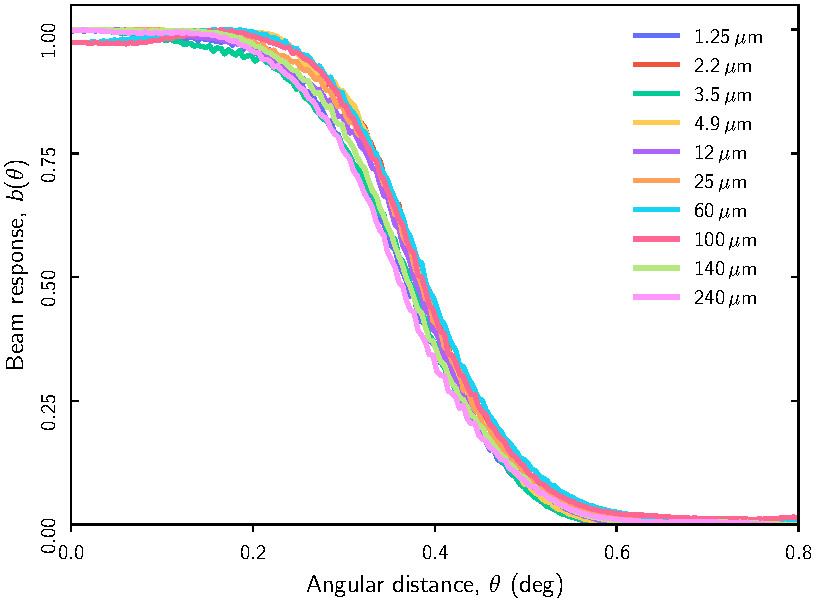
\includegraphics[width=\linewidth]{figs/DIRBE_beam_theta.pdf}\\
  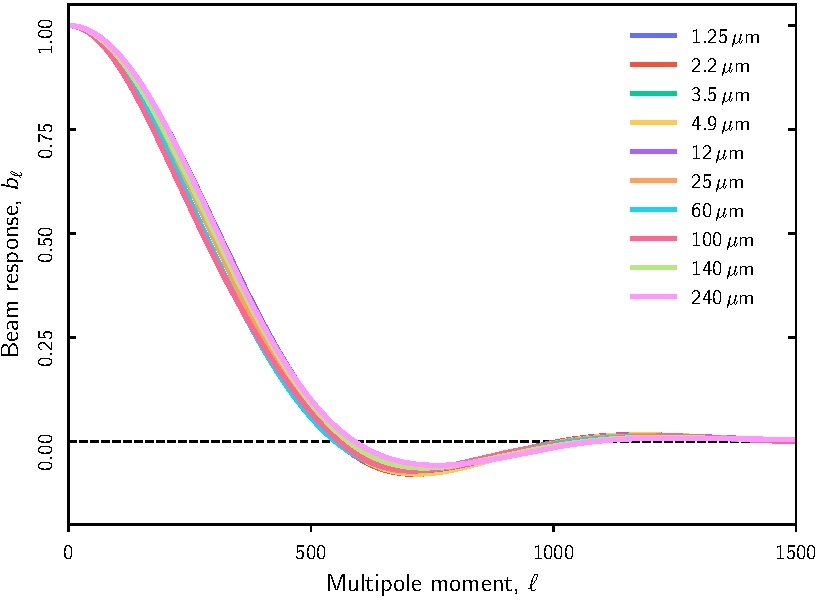
\includegraphics[width=\linewidth]{figs/DIRBE_beam_ell.pdf}
  \caption{Symmetrized beam response functions for each DIRBE channel, both in real space (\emph{top}) and in harmonic space (\emph{bottom}).}
  \label{fig:beams}
\end{figure}

\begin{figure}
  \centering
  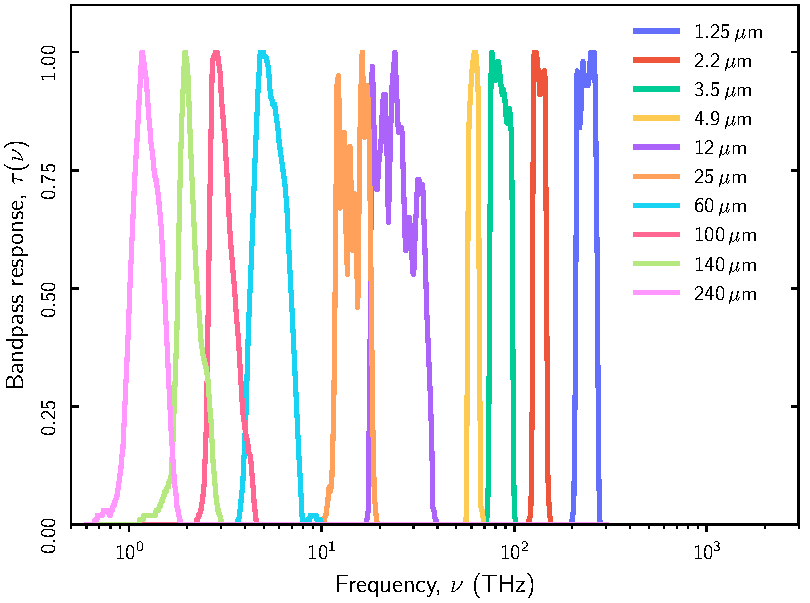
\includegraphics[width=\linewidth]{figs/DIRBE_bp.pdf}
  \caption{Bandpass response functions for each DIRBE channel, plotted as a function of frequency.}
  \label{fig:bandpass}
\end{figure}


\subsection{The DIRBE instrument}

\textit{Duncan: write about the beams. We need nside 512, because nside 256 undersamples}

Discussion about the instrument, picture of the focal plane, etc.


Instead of using the raw time-ordered data, the DIRBE team recommends using the CIOs, which can be though of as a user friendly version of the TODs. The CIOs consist of 1/8th second calibrated observations ordered after pixel numbers. The CIOs were created pre-HEALPix era, and all three experiments aboard \COBE used the Quadrilateralized Spherical Cube pixelization (QUADCUBE) scheme which is an approximately equal-area projection where each pixel lie on one of four cube faces. The DIRBE team did provide us with a script which converts these QUADCUBE pixels into ecliptic longitue and latitude coordinates.
\subsection{DIRBE TOD preprocessing}
\label{sec:tod}
%\subsubsection{DIRBE Calibrated Individual Observations (CIOs)}
%\subsubsection{Quadrilateralized Spherical Cube to HEALPix conversion}
%\subsubsection{Time reordering}
%\subsubsection{Gap-filling}
%\subsubsection{Regenerating planet flags}
%\subsection{Publicly available DIRBE products}





\begin{figure*}
  \centering
   	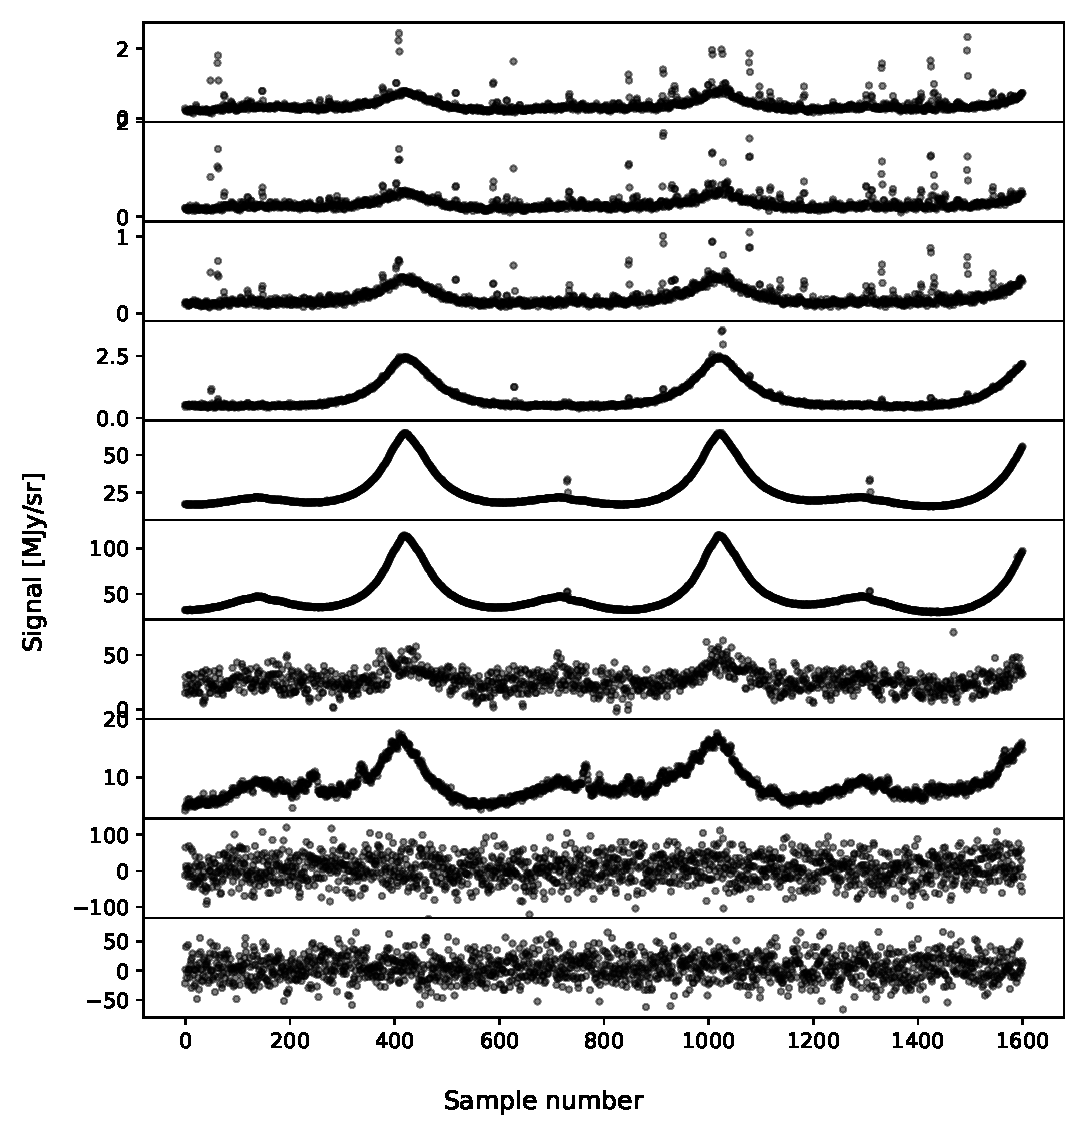
\includegraphics[width=\linewidth]{figs/cios.pdf}
  	\caption{Time-ordered data segment of each DIRBE band (1-10) from top to bottom.}
	\label{fig: cios}
\end{figure*}




\subsection{Ancillary data sets}

\subsubsection{Planck HFI}

\subsubsection{WISE and GAIA}

\subsubsection{COBE-FIRAS}

\textit{Duncan will write this section too}


\section{Data selection and goodness-of-fit}
\label{sec:data_selection}

\subsection{Baseline data selection}

\subsection{Mask definitions}

\begin{figure}
  \centering
  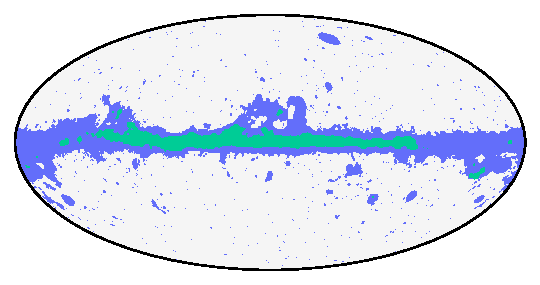
\includegraphics[width=\columnwidth]{figs/mask_proc_calib.pdf}
  \caption{Processing masks use in the analysis.}
  \label{fig:masks}
\end{figure}


\subsubsection{Galactic masks}

\subsubsection{Solar-centered residual masks}

\subsection{Goodness-of-fit statistics}

\subsection{Summary of included data}


\clearpage
\section{Low-level posterior distributions}
\label{sec:posteriors}

\begin{figure*}
	\centering
	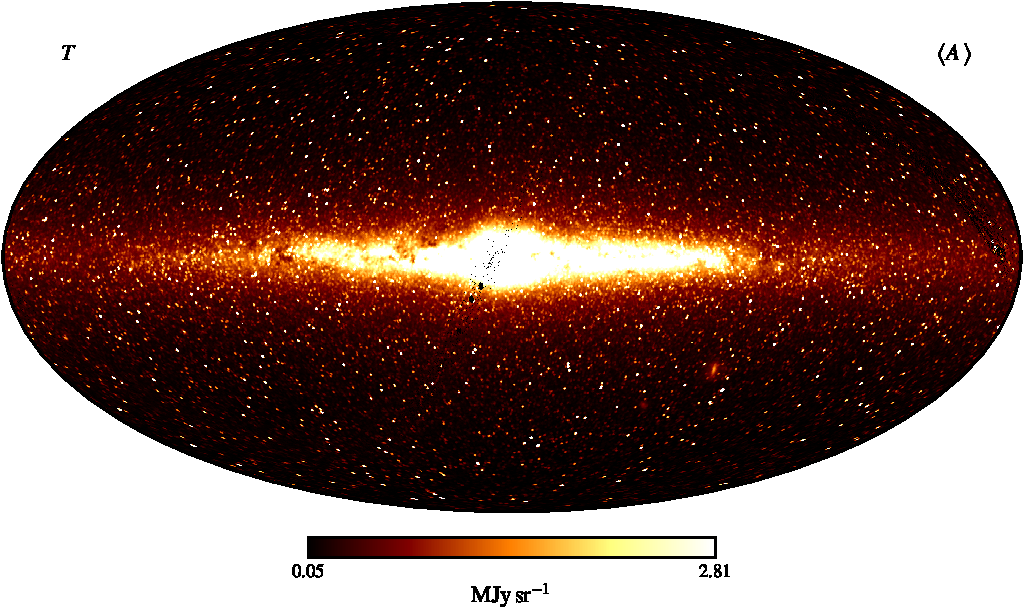
\includegraphics[width=0.58\linewidth]{figs/CG_DIRBE_01_n0512_DR2_I_MEAN_w18_n512_cb_c-afmhot.pdf}\\
        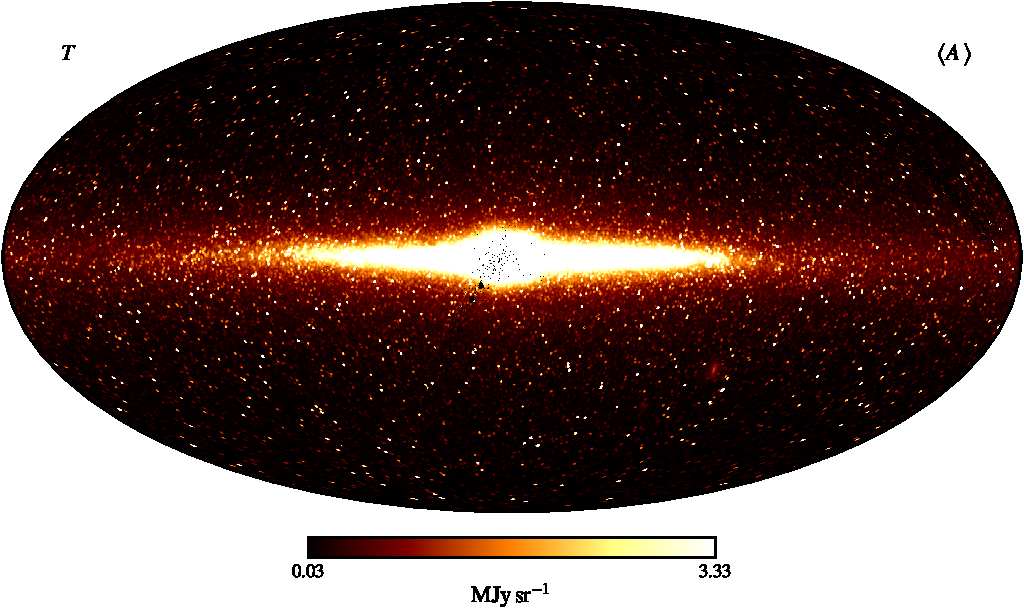
\includegraphics[width=0.58\linewidth]{figs/CG_DIRBE_02_n0512_DR2_I_MEAN_w18_n512_cb_c-afmhot.pdf}\\
        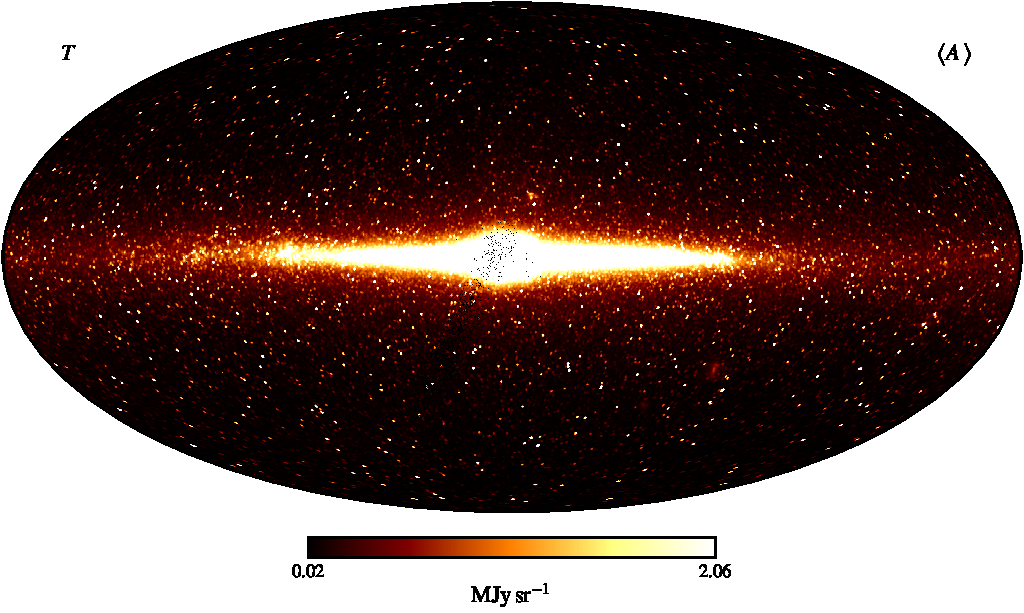
\includegraphics[width=0.58\linewidth]{figs/CG_DIRBE_03_n0512_DR2_I_MEAN_w18_n512_cb_c-afmhot.pdf}\\
        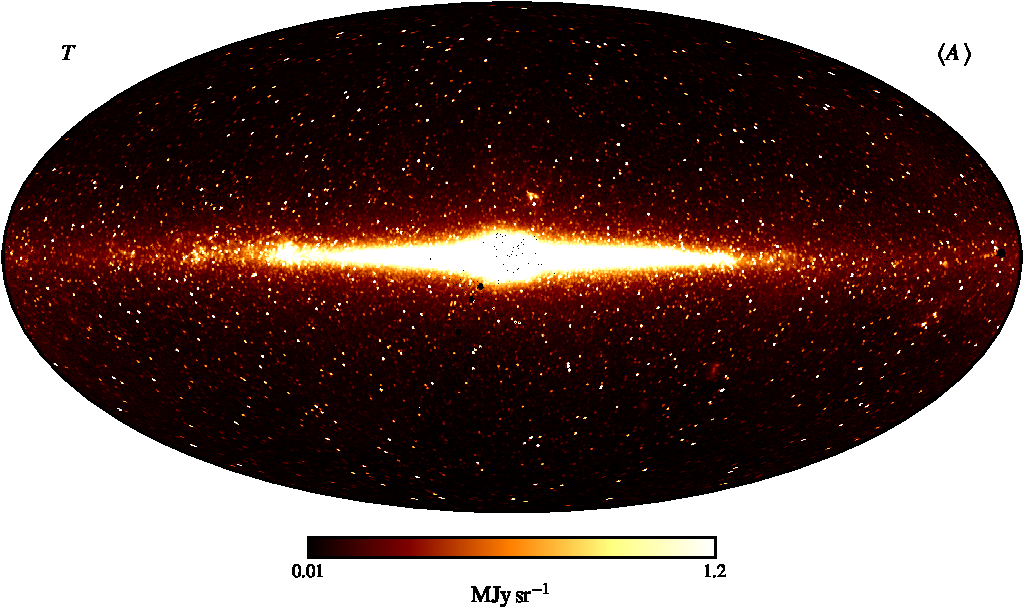
\includegraphics[width=0.58\linewidth]{figs/CG_DIRBE_04_n0512_DR2_I_MEAN_w18_n512_cb_c-afmhot.pdf}
	\caption{}
	\label{fig:freqmaps1_4}
\end{figure*}

\begin{figure*}
	\centering
	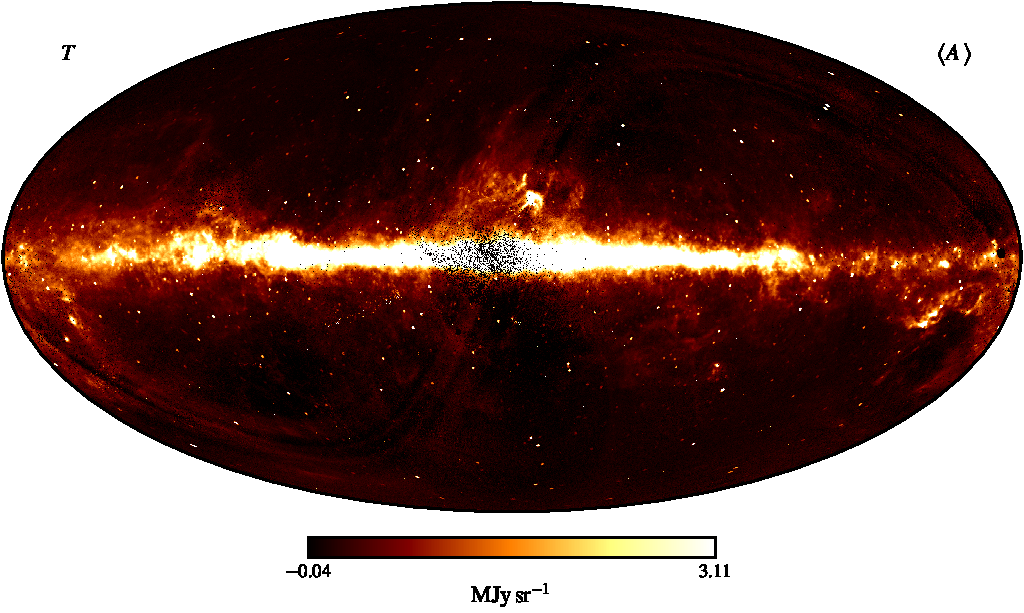
\includegraphics[width=0.73\linewidth]{figs/CG_DIRBE_05_n0512_DR2_I_MEAN_w18_n512_cb_c-afmhot.pdf}\\
        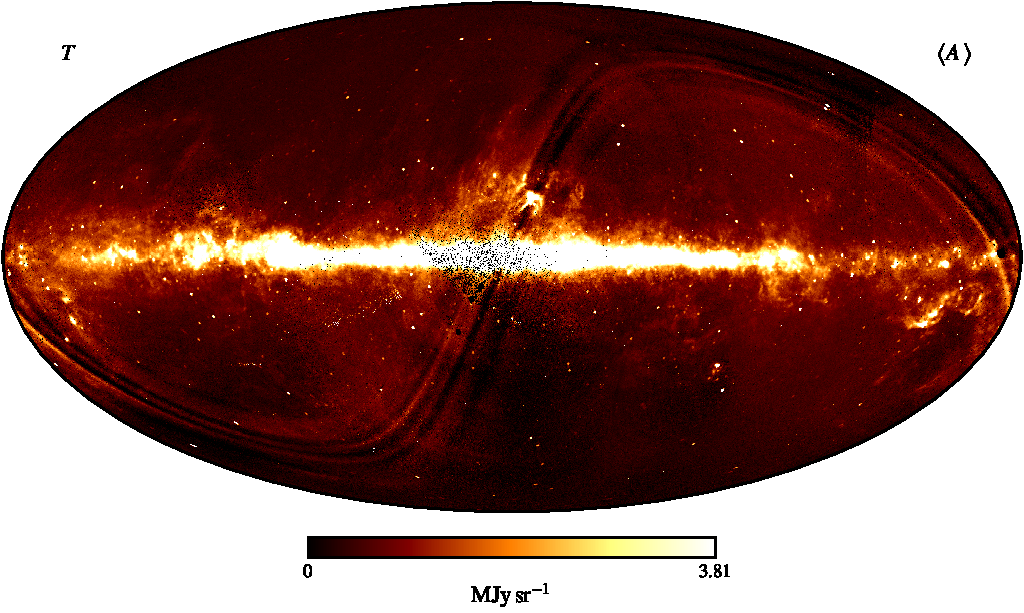
\includegraphics[width=0.73\linewidth]{figs/CG_DIRBE_06_n0512_DR2_I_MEAN_w18_n512_cb_c-afmhot.pdf}\\
        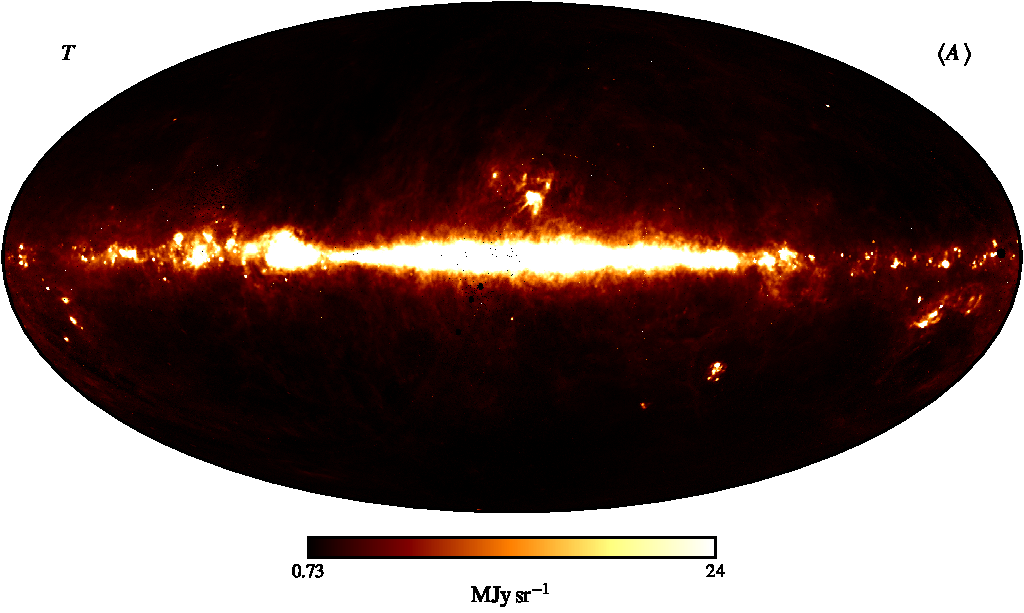
\includegraphics[width=0.73\linewidth]{figs/CG_DIRBE_07_n0512_DR2_I_MEAN_w18_n512_cb_c-afmhot.pdf}
	\caption{}
	\label{fig:freqmaps5_7}
\end{figure*}

\begin{figure*}
	\centering
        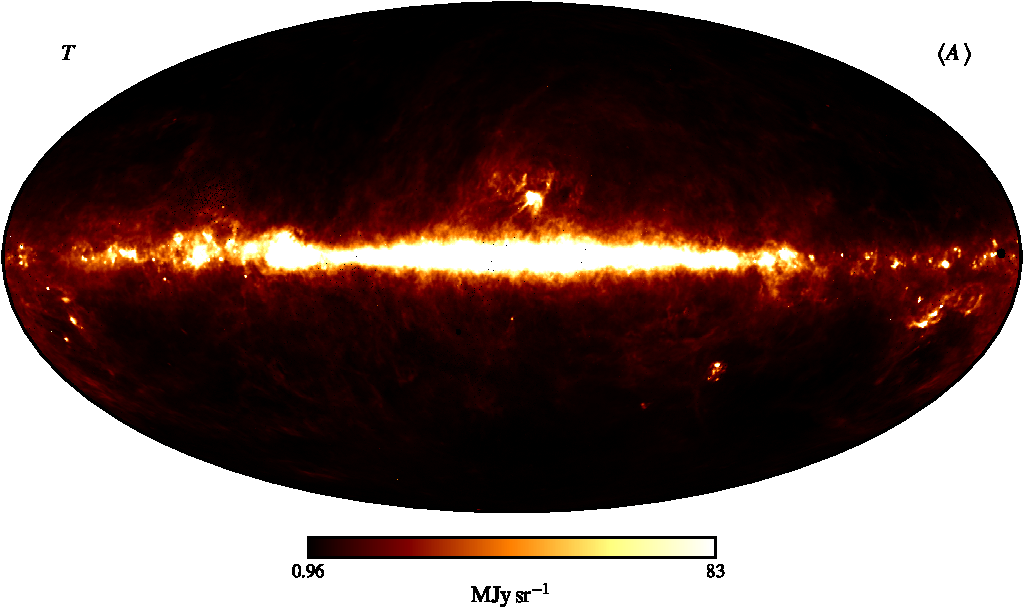
\includegraphics[width=0.73\linewidth]{figs/CG_DIRBE_08_n0512_DR2_I_MEAN_w18_n512_cb_c-afmhot.pdf}\\
        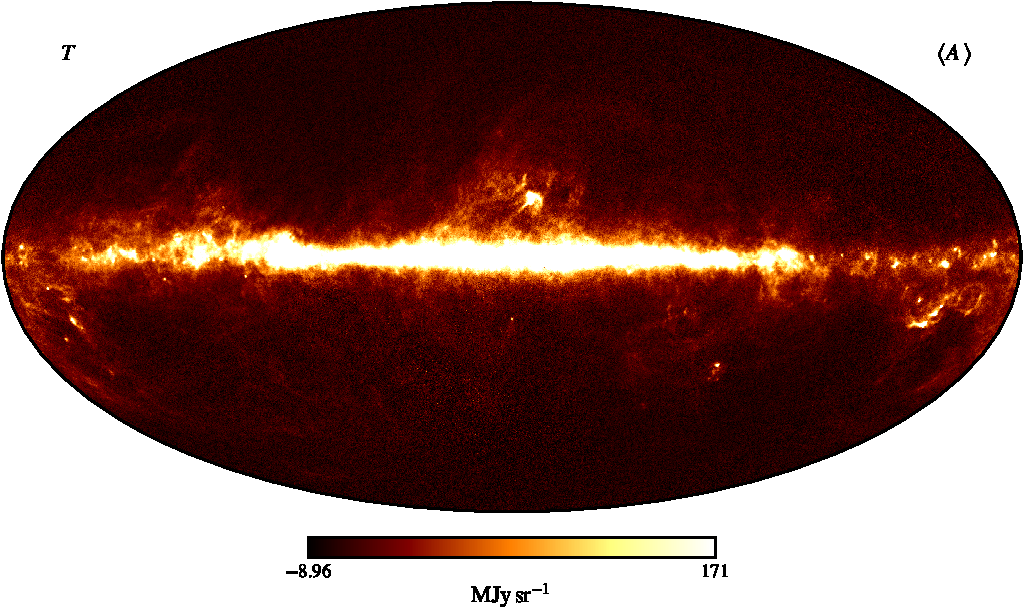
\includegraphics[width=0.73\linewidth]{figs/CG_DIRBE_09_n0512_DR2_I_MEAN_w18_n512_cb_c-afmhot.pdf}\\
        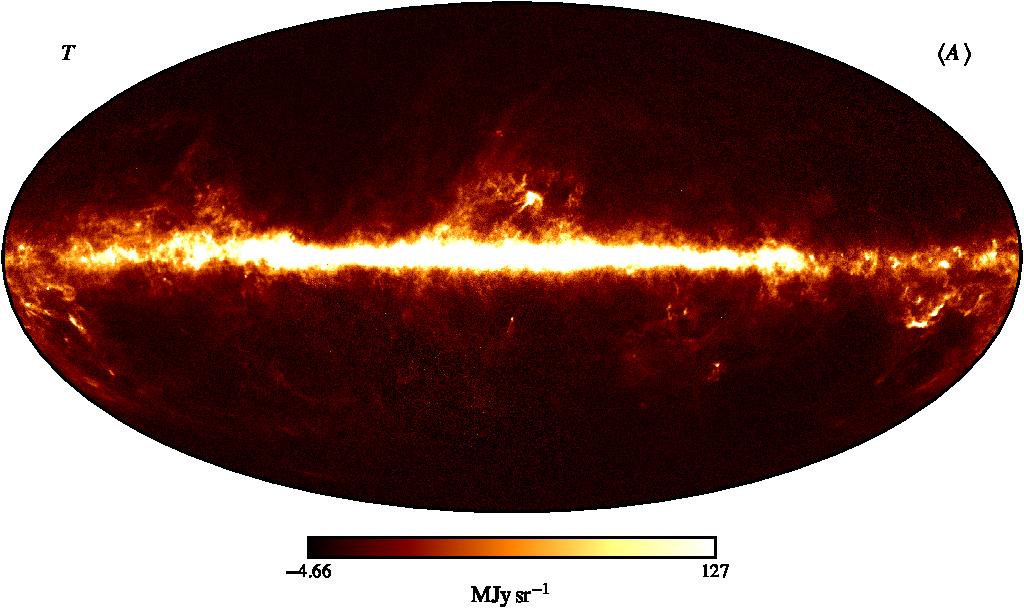
\includegraphics[width=0.73\linewidth]{figs/CG_DIRBE_10_n0512_DR2_I_MEAN_w18_n512_cb_c-afmhot.pdf}
	\caption{}
	\label{fig:freqmaps8_10}
\end{figure*}

\begin{figure*}
	\centering
	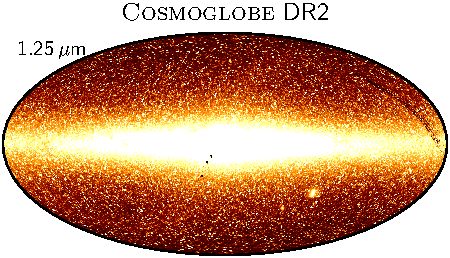
\includegraphics[width=0.23\linewidth]{figs/CG_DIRBE_01_I_n0256_DR2.pdf}
        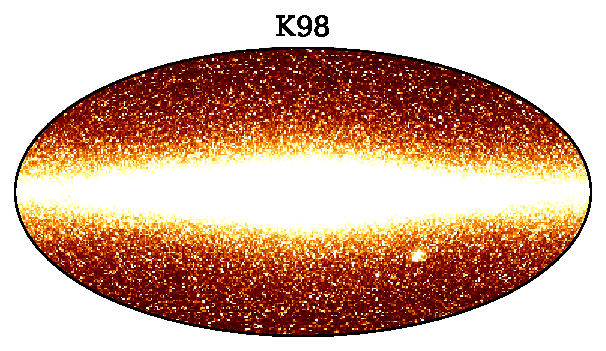
\includegraphics[width=0.23\linewidth]{figs/DIRBE_ZSMA_01_1_256.pdf}
        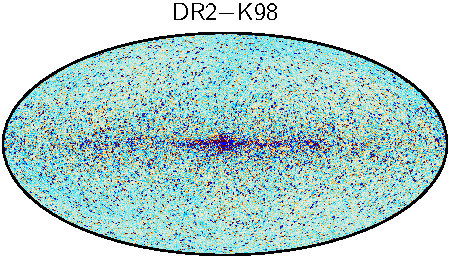
\includegraphics[width=0.23\linewidth]{figs/diff_CG_DIRBE_ZSMA_01_n256.pdf}\\
	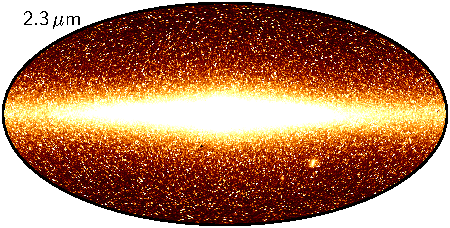
\includegraphics[width=0.23\linewidth]{figs/CG_DIRBE_02_I_n0256_DR2.pdf}
        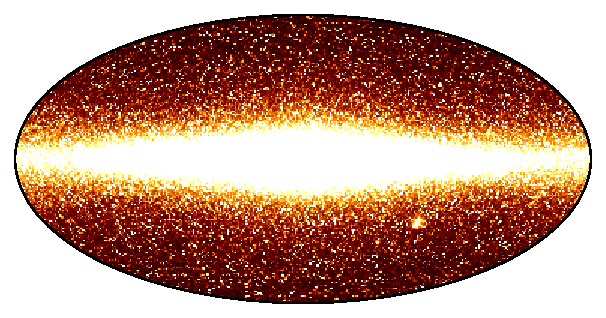
\includegraphics[width=0.23\linewidth]{figs/DIRBE_ZSMA_02_1_256.pdf}
        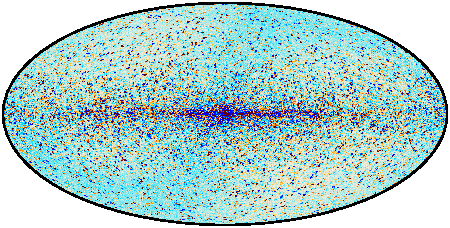
\includegraphics[width=0.23\linewidth]{figs/diff_CG_DIRBE_ZSMA_02_n256.pdf}\\
	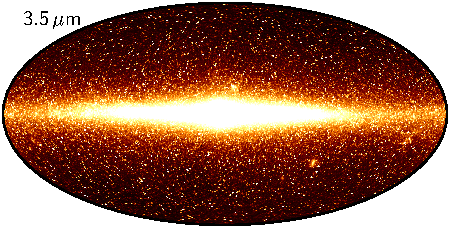
\includegraphics[width=0.23\linewidth]{figs/CG_DIRBE_03_I_n0256_DR2.pdf}
        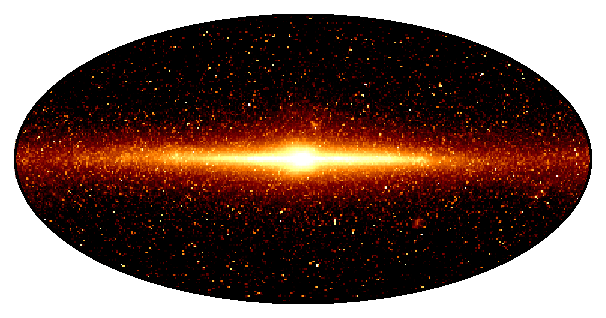
\includegraphics[width=0.23\linewidth]{figs/DIRBE_ZSMA_03_1_256.pdf}
        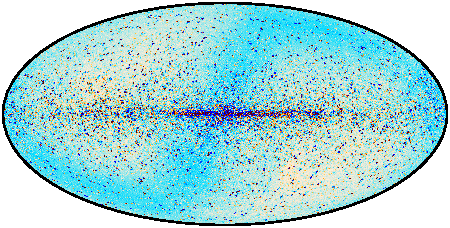
\includegraphics[width=0.23\linewidth]{figs/diff_CG_DIRBE_ZSMA_03_n256.pdf}\\
	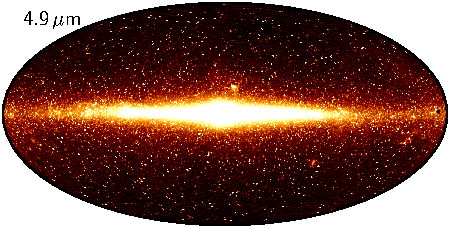
\includegraphics[width=0.23\linewidth]{figs/CG_DIRBE_04_I_n0256_DR2.pdf}
        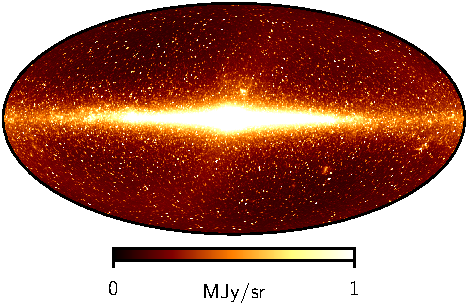
\includegraphics[width=0.23\linewidth]{figs/DIRBE_ZSMA_04_1_256.pdf}
        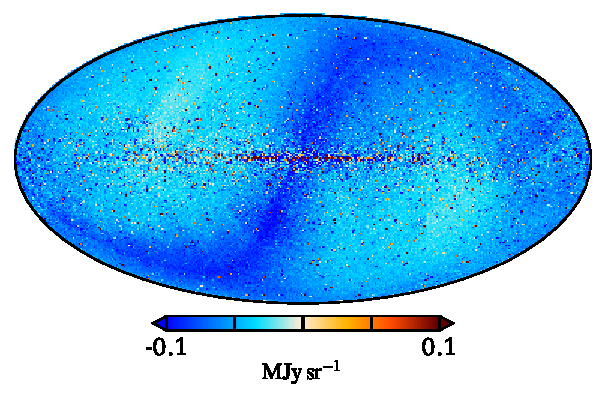
\includegraphics[width=0.23\linewidth]{figs/diff_CG_DIRBE_ZSMA_04_n256.pdf}\\
	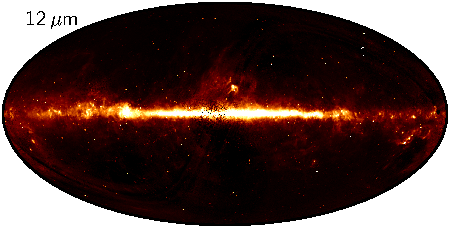
\includegraphics[width=0.23\linewidth]{figs/CG_DIRBE_05_I_n0256_DR2.pdf}
        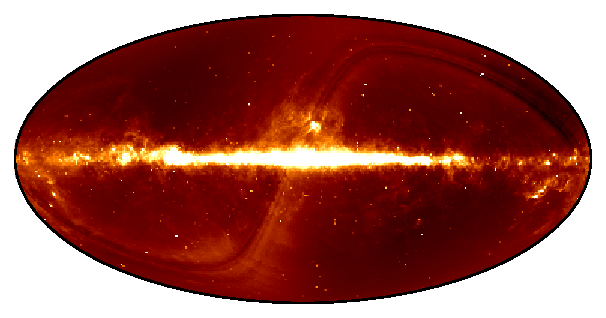
\includegraphics[width=0.23\linewidth]{figs/DIRBE_ZSMA_05_1_256.pdf}
        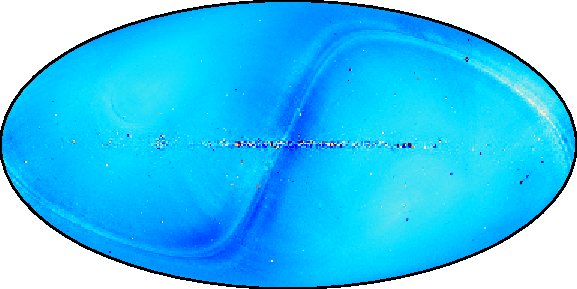
\includegraphics[width=0.23\linewidth]{figs/diff_CG_DIRBE_ZSMA_05_n256.pdf}\\
	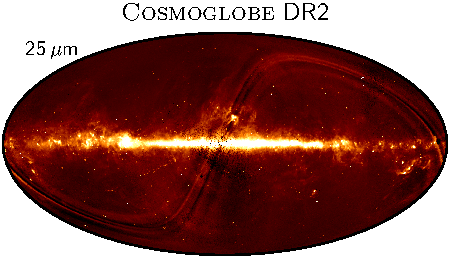
\includegraphics[width=0.23\linewidth]{figs/CG_DIRBE_06_I_n0256_DR2.pdf}
        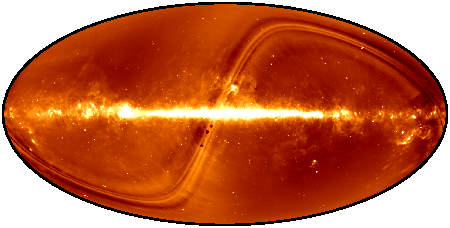
\includegraphics[width=0.23\linewidth]{figs/DIRBE_ZSMA_06_1_256.pdf}
        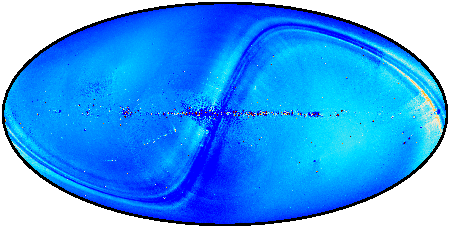
\includegraphics[width=0.23\linewidth]{figs/diff_CG_DIRBE_ZSMA_06_n256.pdf}\\
	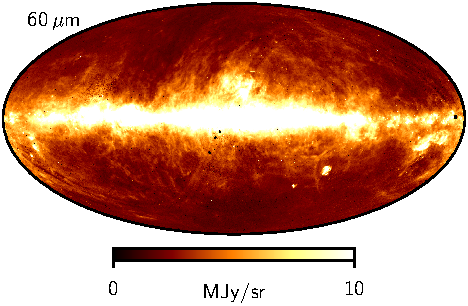
\includegraphics[width=0.23\linewidth]{figs/CG_DIRBE_07_I_n0256_DR2.pdf}
        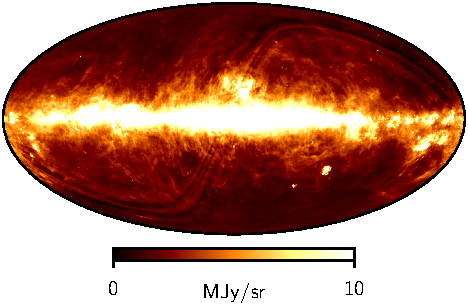
\includegraphics[width=0.23\linewidth]{figs/DIRBE_ZSMA_07_1_256.pdf}
        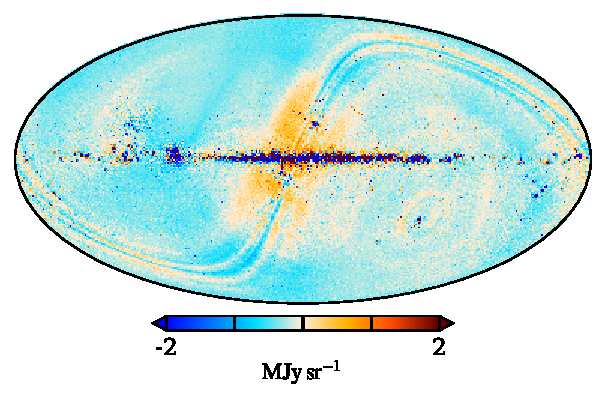
\includegraphics[width=0.23\linewidth]{figs/diff_CG_DIRBE_ZSMA_07_n256.pdf}\\
	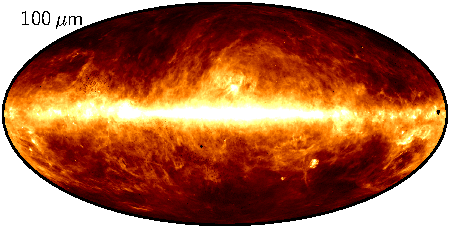
\includegraphics[width=0.23\linewidth]{figs/CG_DIRBE_08_I_n0256_DR2.pdf}
        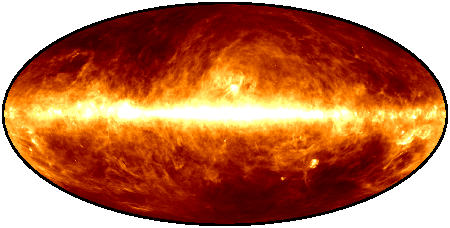
\includegraphics[width=0.23\linewidth]{figs/DIRBE_ZSMA_08_1_256.pdf}
        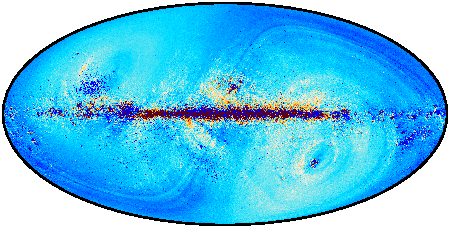
\includegraphics[width=0.23\linewidth]{figs/diff_CG_DIRBE_ZSMA_08_n256.pdf}\\
        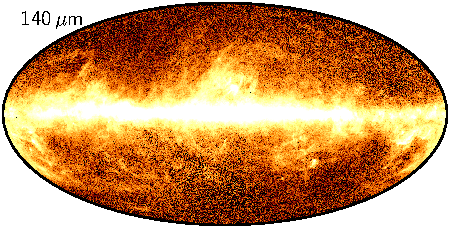
\includegraphics[width=0.23\linewidth]{figs/CG_DIRBE_09_I_n0256_DR2.pdf}
        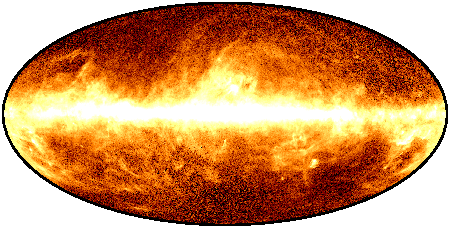
\includegraphics[width=0.23\linewidth]{figs/DIRBE_ZSMA_09_1_256.pdf}
        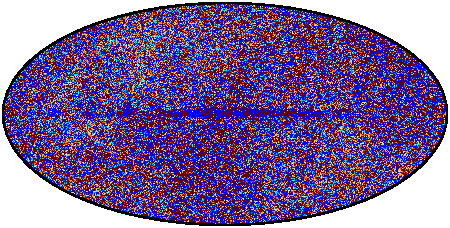
\includegraphics[width=0.23\linewidth]{figs/diff_CG_DIRBE_ZSMA_09_n256.pdf}\\
        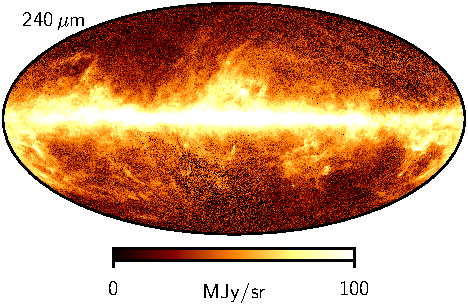
\includegraphics[width=0.23\linewidth]{figs/CG_DIRBE_10_I_n0256_DR2.pdf}
        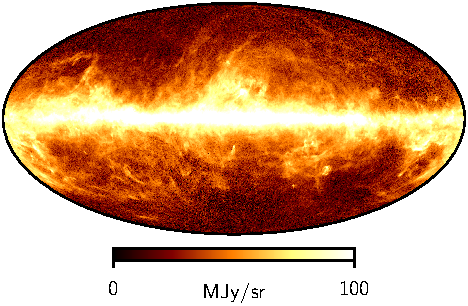
\includegraphics[width=0.23\linewidth]{figs/DIRBE_ZSMA_10_1_256.pdf}
        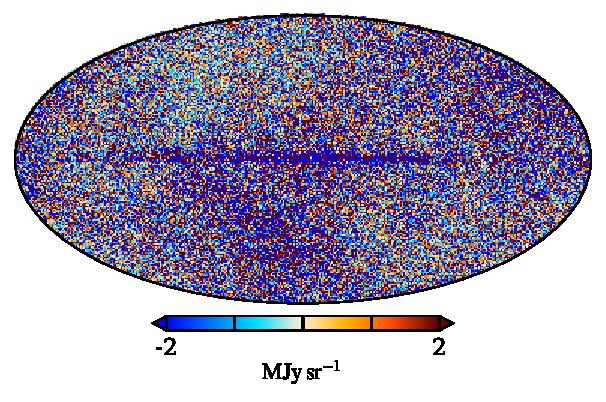
\includegraphics[width=0.23\linewidth]{figs/diff_CG_DIRBE_ZSMA_10_n256.pdf}\\
	\caption{Comparison of \Cosmoglobe\ DR2 (\emph{left column}) and legacy DIRBE (\emph{middle column}) zodiacal light subtracted mission average maps. Difference maps are shown in the rightmost column. Full maps are plotted with a non-linear and strictly positive color range, while difference maps are plotted with a linear and symmetric color range.   }
	\label{fig:freqmaps_cg_vs_dirbe}
\end{figure*}

%\begin{figure*}
%	\centering
%	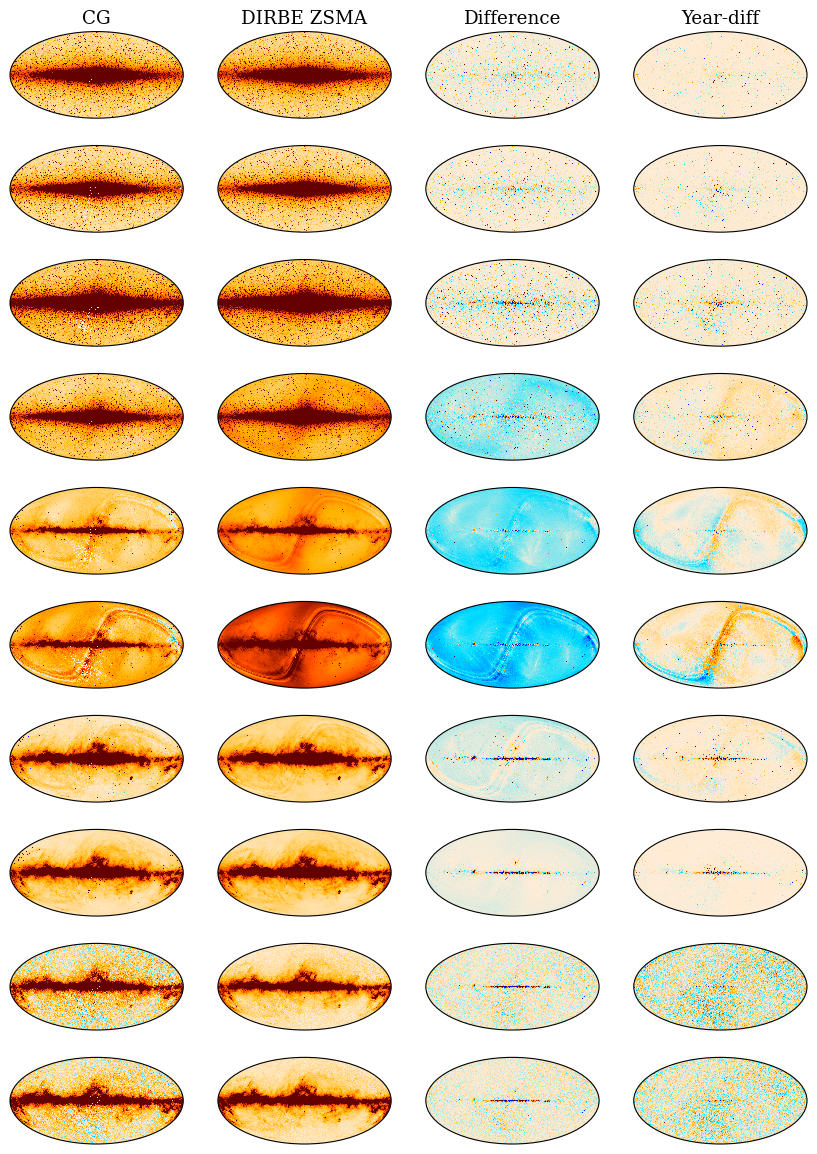
\includegraphics[width=\linewidth]{figs/diff_grid.png}
	% Figure to make this script is currently in /mn/stornext/d5/data/duncanwa/DIRBE/plots/diff_grid.py
%	\caption{Cosmoglobe, DIRBE ZSMA official maps, their difference, and the internal halfmission splits for Cosmoglobe.}
%	\label{fig:diff_grid}
%\end{figure*}


\subsection{Instrumental noise}

\subsection{Calibration}

\subsection{Beam characterization}

\begin{figure}
	\centering
	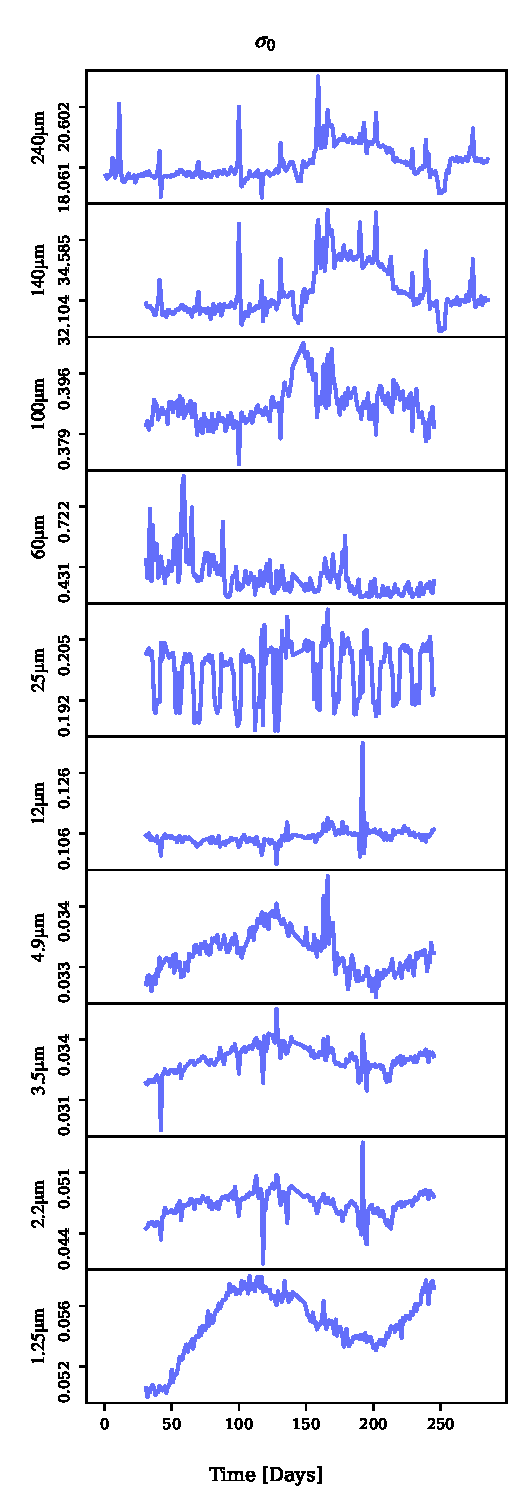
\includegraphics[width=\columnwidth]{figs/sigma0_bands.pdf}
	\caption{Sigma0 for each band}
	\label{fig:sigma0}
\end{figure}

\begin{figure}
	\centering
	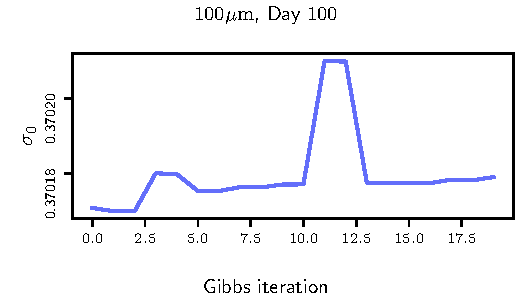
\includegraphics[width=\columnwidth]{figs/sigma0_trace.pdf}
	\caption{Sigma0 for scan 100}
	\label{fig:sigma0_band8}
\end{figure}

\begin{figure}
	\centering
	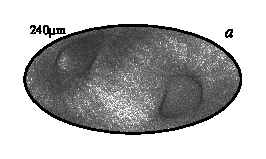
\includegraphics{figs/rms_maps/rms_10a_c0001_000022.pdf}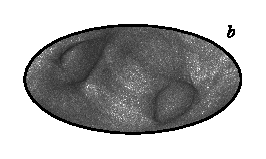
\includegraphics{figs/rms_maps/rms_10b_c0001_000022.pdf}
  \vspace*{-0.85cm}

	\includegraphics{figs/rms_maps/rms_09a_c0001_000022.pdf}\includegraphics{figs/rms_maps/rms_09b_c0001_000022.pdf}
  \vspace*{-0.85cm}

	\includegraphics{figs/rms_maps/rms_08a_c0001_000022.pdf}\includegraphics{figs/rms_maps/rms_08b_c0001_000022.pdf}
  \vspace*{-0.85cm}

	\includegraphics{figs/rms_maps/rms_07a_c0001_000022.pdf}\includegraphics{figs/rms_maps/rms_07b_c0001_000022.pdf}
  \vspace*{-0.85cm}

	\includegraphics{figs/rms_maps/rms_06a_c0001_000022.pdf}\includegraphics{figs/rms_maps/rms_06b_c0001_000022.pdf}
  \vspace*{-0.85cm}

	\includegraphics{figs/rms_maps/rms_05a_c0001_000022.pdf}\includegraphics{figs/rms_maps/rms_05b_c0001_000022.pdf}
  \vspace*{-0.85cm}

	\includegraphics{figs/rms_maps/rms_04a_c0001_000022.pdf}\includegraphics{figs/rms_maps/rms_04b_c0001_000022.pdf}
  \vspace*{-0.85cm}

	\includegraphics{figs/rms_maps/rms_03a_c0001_000022.pdf}\includegraphics{figs/rms_maps/rms_03b_c0001_000022.pdf}
  \vspace*{-0.85cm}

	\includegraphics{figs/rms_maps/rms_02a_c0001_000022.pdf}\includegraphics{figs/rms_maps/rms_02b_c0001_000022.pdf}
  \vspace*{-0.85cm}

	\includegraphics{figs/rms_maps/rms_01a_c0001_000022.pdf}\includegraphics{figs/rms_maps/rms_01b_c0001_000022.pdf}
  \vspace*{-0.85cm}

	\caption{Cosmoglobe halfmission split white noise RMS for each band. The color scales are (0, 0.02) MJy/sr for bands 1-4, (0, 0.1) for bands 4-6, (0, 0.4) for bands 6-8, and (0, 20) for bands 8-10}
	\label{fig:rms}
\end{figure}

\begin{figure}
  % script to make these are in /mn/stornext/u3/metins/dirbe/DR2/plot_maps.py (cosmoglobe_analysis_plotter.plot_ncorr_maps(sample=19))
	\centering
	\includegraphics{figs/ncorr_10_c0001_000022.pdf}
  \vspace{-1cm}
  
	\includegraphics{figs/ncorr_09_c0001_000022.pdf}
  \vspace{-0.2cm}
  
	\includegraphics[width=0.5\columnwidth]{figs/ncorr_cbar_c0001_000019.pdf}

	\caption{Correlated noise maps (inverse-variance-weighted of half-mission splits) for bands 9 and 10. The other bands are not clean enought for correlated noise fitting.}
	\label{fig:ncorr}
\end{figure}

%\begin{figure*}

%  \centering
%    \includegraphics[width=0.8\columnwidth]{figs/freq_maps/freq_01_c0001_000022.pdf}\includegraphics[width=0.8\columnwidth]{figs/freq_maps/freq_06_c0001_000022.pdf}
    % \vspace*{-0.5cm}

%    \includegraphics[width=0.4\columnwidth]{figs/freq_maps/freq_cbar_01_c0001_000022.pdf}\hspace{3.6cm}\includegraphics[width=0.4\columnwidth]{figs/freq_maps/freq_cbar_06_c0001_000022.pdf}

%    \includegraphics[width=0.8\columnwidth]{figs/freq_maps/freq_02_c0001_000022.pdf}\includegraphics[width=0.8\columnwidth]{figs/freq_maps/freq_07_c0001_000022.pdf}
    % \vspace*{-0.5cm}

%    \includegraphics[width=0.4\columnwidth]{figs/freq_maps/freq_cbar_02_c0001_000022.pdf}\hspace{3.6cm}\includegraphics[width=0.4\columnwidth]{figs/freq_maps/freq_cbar_07_c0001_000022.pdf}

  
%    \includegraphics[width=0.8\columnwidth]{figs/freq_maps/freq_03_c0001_000022.pdf}\includegraphics[width=0.8\columnwidth]{figs/freq_maps/freq_08_c0001_000022.pdf}
    % \vspace*{-0.5cm}

%    \includegraphics[width=0.4\columnwidth]{figs/freq_maps/freq_cbar_03_c0001_000022.pdf}\hspace{3.6cm}\includegraphics[width=0.4\columnwidth]{figs/freq_maps/freq_cbar_08_c0001_000022.pdf}

  
%    \includegraphics[width=0.8\columnwidth]{figs/freq_maps/freq_04_c0001_000022.pdf}\includegraphics[width=0.8\columnwidth]{figs/freq_maps/freq_09_c0001_000022.pdf}
    % \vspace*{-0.5cm}

%    \includegraphics[width=0.4\columnwidth]{figs/freq_maps/freq_cbar_04_c0001_000022.pdf}\hspace{3.6cm}\includegraphics[width=0.4\columnwidth]{figs/freq_maps/freq_cbar_09_c0001_000022.pdf}

  
%    \includegraphics[width=0.8\columnwidth]{figs/freq_maps/freq_05_c0001_000022.pdf}\includegraphics[width=0.8\columnwidth]{figs/freq_maps/freq_10_c0001_000022.pdf}
    % \vspace*{-0.5cm}

%    \includegraphics[width=0.4\columnwidth]{figs/freq_maps/freq_cbar_05_c0001_000022.pdf}\hspace{3.6cm}\includegraphics[width=0.4\columnwidth]{figs/freq_maps/freq_cbar_10_c0001_000022.pdf}

  
  
%    \caption{Frequency maps}
%    \label{fig:freq_maps}
%\end{figure*}

\section{Frequency maps}
\label{sec:maps}

\subsection{ZSMA frequency maps}

\subsection{Residual maps}

\subsection{Half-mission difference maps}

\subsection{Comparison with official DIRBE products}



\clearpage
\section{\Cosmoglobe\ Data Release 2}
\label{sec:astrophysics}

\subsection{Frequency maps}

\subsection{Zodiacal light emission}

\clearpage
\subsection{Galactic emission}

\begin{figure*}
	\centering
	\includegraphics[width=0.49\linewidth]{figs/CG_dust_v05_I_MEAN_w12_n2048_cb_c-sunburst.pdf}
        \includegraphics[width=0.49\linewidth]{figs/CG_CO_tot_v05_I_MEAN_w12_n1024_cb_c-afmhot.pdf}\\
        \includegraphics[width=0.49\linewidth]{figs/CG_freefree_v05_I_MEAN_w12_n1024_cb_c-freeze.pdf}
        \includegraphics[width=0.49\linewidth]{figs/CG_stars_n0512_v06_I_MEAN_w12_n512_cb_c-afmhot.pdf}\\
	\caption{}
	\label{fig:fg_amp}
\end{figure*}

\begin{figure*}
  \centering
  \includegraphics[width=0.19\linewidth]{figs/compfreq_mapzodi_10a_v01.pdf}
  \includegraphics[width=0.19\linewidth]{figs/compfreq_zodi_10a_v01.pdf}
  \includegraphics[width=0.19\linewidth]{figs/compfreq_dusttot_10a_v01.pdf}
  \includegraphics[width=0.19\linewidth]{figs/compfreq_white_nobar.pdf}  
  \includegraphics[width=0.19\linewidth]{figs/compfreq_todres_10a_v01.pdf}\\
  \includegraphics[width=0.19\linewidth]{figs/compfreq_mapzodi_09a_v01.pdf}
  \includegraphics[width=0.19\linewidth]{figs/compfreq_zodi_09a_v01.pdf}
  \includegraphics[width=0.19\linewidth]{figs/compfreq_dusttot_09a_v01.pdf}
  \includegraphics[width=0.19\linewidth]{figs/compfreq_white_nobar.pdf}  
  \includegraphics[width=0.19\linewidth]{figs/compfreq_todres_09a_v01.pdf}\\
  \includegraphics[width=0.19\linewidth]{figs/compfreq_mapzodi_08a_v01.pdf}
  \includegraphics[width=0.19\linewidth]{figs/compfreq_zodi_08a_v01.pdf}
  \includegraphics[width=0.19\linewidth]{figs/compfreq_dusttot_08a_v01.pdf}
  \includegraphics[width=0.19\linewidth]{figs/compfreq_white_nobar.pdf}  
  \includegraphics[width=0.19\linewidth]{figs/compfreq_todres_08a_v01.pdf}\\
  \includegraphics[width=0.19\linewidth]{figs/compfreq_mapzodi_07a_v01.pdf}
  \includegraphics[width=0.19\linewidth]{figs/compfreq_zodi_07a_v01.pdf}
  \includegraphics[width=0.19\linewidth]{figs/compfreq_dusttot_07a_v01.pdf}
  \includegraphics[width=0.19\linewidth]{figs/compfreq_white_nobar.pdf}  
  \includegraphics[width=0.19\linewidth]{figs/compfreq_todres_07a_v01.pdf}\\
  \includegraphics[width=0.19\linewidth]{figs/compfreq_mapzodi_06a_v01.pdf}
  \includegraphics[width=0.19\linewidth]{figs/compfreq_zodi_06a_v01.pdf}
  \includegraphics[width=0.19\linewidth]{figs/compfreq_dusttot_06a_v01.pdf}
  \includegraphics[width=0.19\linewidth]{figs/compfreq_stars_06a_v01.pdf}  
  \includegraphics[width=0.19\linewidth]{figs/compfreq_todres_06a_v01.pdf}\\  
  \includegraphics[width=0.19\linewidth]{figs/compfreq_mapzodi_05a_v01.pdf}
  \includegraphics[width=0.19\linewidth]{figs/compfreq_zodi_05a_v01.pdf}
  \includegraphics[width=0.19\linewidth]{figs/compfreq_dusttot_05a_v01.pdf}
  \includegraphics[width=0.19\linewidth]{figs/compfreq_stars_05a_v01.pdf}  
  \includegraphics[width=0.19\linewidth]{figs/compfreq_todres_05a_v01.pdf}\\
  \includegraphics[width=0.19\linewidth]{figs/compfreq_mapzodi_04a_v01.pdf}
  \includegraphics[width=0.19\linewidth]{figs/compfreq_zodi_04a_v01.pdf}
  \includegraphics[width=0.19\linewidth]{figs/compfreq_white_nobar.pdf}
  \includegraphics[width=0.19\linewidth]{figs/compfreq_stars_04a_v01.pdf}  
  \includegraphics[width=0.19\linewidth]{figs/compfreq_todres_04a_v01.pdf}\\  
  \includegraphics[width=0.19\linewidth]{figs/compfreq_mapzodi_03a_v01.pdf}
  \includegraphics[width=0.19\linewidth]{figs/compfreq_zodi_03a_v01.pdf}
  \includegraphics[width=0.19\linewidth]{figs/compfreq_white_nobar.pdf}
  \includegraphics[width=0.19\linewidth]{figs/compfreq_stars_03a_v01.pdf}  
  \includegraphics[width=0.19\linewidth]{figs/compfreq_todres_03a_v01.pdf}\\  
  \includegraphics[width=0.19\linewidth]{figs/compfreq_mapzodi_02a_v01.pdf}
  \includegraphics[width=0.19\linewidth]{figs/compfreq_zodi_02a_v01.pdf}
  \includegraphics[width=0.19\linewidth]{figs/compfreq_white_nobar.pdf}
  \includegraphics[width=0.19\linewidth]{figs/compfreq_stars_02a_v01.pdf}  
  \includegraphics[width=0.19\linewidth]{figs/compfreq_todres_02a_v01.pdf}\\
  \includegraphics[width=0.19\linewidth]{figs/compfreq_mapzodi_01a_v01.pdf}
  \includegraphics[width=0.19\linewidth]{figs/compfreq_zodi_01a_v01.pdf}
  \includegraphics[width=0.19\linewidth]{figs/compfreq_white_nobar.pdf}
  \includegraphics[width=0.19\linewidth]{figs/compfreq_stars_01a_v01.pdf}
  \includegraphics[width=0.19\linewidth]{figs/compfreq_todres_01a_v01.pdf}\\
  \includegraphics[width=0.50\linewidth]{figs/colourbar_MJysr.pdf}
  \caption{Comparison between the raw DIRBE data and the various fitted components for one single Gibbs sample. Columns show, from left to right, 1) the time-ordered DIRBE data co-added into pixelized maps; 2) zodiacal light emission; 3) thermal dust emission; 4) star emission; and 5) data-minus-model residual emission. Rows show individual frequency channels. Missing entries corresponds to components that are forced to zero in the model. Note that all panels are plotted with the same color scale in units of MJy/sr, and can be directly compared.}
  \label{fig:comp_vs_freq}
\end{figure*}

\begin{figure*}
	\centering
	\includegraphics[width=\textwidth]{figs/all_fgs.pdf}
	\caption{Summary of all foregrounds.}
	\label{fig:SED_overview}
\end{figure*}


\clearpage
%\subsection{Goodness-of-fit and residual maps}


\begin{figure}
	\centering
	\includegraphics{figs/chisq_total.pdf}
	\includegraphics{figs/chisq_total_cbar.pdf}
	\caption{Pixel-space reduced normalized $\chi^2$.}
	\label{fig:chisq}
\end{figure}

\begin{figure}
	\centering
	\includegraphics{figs/res_maps/res_10a_c0001_000022.pdf}\includegraphics{figs/res_maps/res_10b_c0001_000022.pdf}
  \vspace*{-0.85cm}

	\includegraphics{figs/res_maps/res_09a_c0001_000022.pdf}\includegraphics{figs/res_maps/res_09b_c0001_000022.pdf}
  \vspace*{-0.85cm}

	\includegraphics{figs/res_maps/res_08a_c0001_000022.pdf}\includegraphics{figs/res_maps/res_08b_c0001_000022.pdf}
  \vspace*{-0.85cm}

	\includegraphics{figs/res_maps/res_07a_c0001_000022.pdf}\includegraphics{figs/res_maps/res_07b_c0001_000022.pdf}
  \vspace*{-0.85cm}

	\includegraphics{figs/res_maps/res_06a_c0001_000022.pdf}\includegraphics{figs/res_maps/res_06b_c0001_000022.pdf}
  \vspace*{-0.85cm}

	\includegraphics{figs/res_maps/res_05a_c0001_000022.pdf}\includegraphics{figs/res_maps/res_05b_c0001_000022.pdf}
  \vspace*{-0.85cm}
  
  \includegraphics{figs/res_maps/res_04a_c0001_000022.pdf}\includegraphics{figs/res_maps/res_04b_c0001_000022.pdf}
  \vspace*{-0.85cm}
  
  \includegraphics{figs/res_maps/res_03a_c0001_000022.pdf}\includegraphics{figs/res_maps/res_03b_c0001_000022.pdf}
  \vspace*{-0.85cm}  

	\includegraphics{figs/res_maps/res_02a_c0001_000022.pdf}\includegraphics{figs/res_maps/res_02b_c0001_000022.pdf}
  \vspace*{-0.85cm}

	\includegraphics{figs/res_maps/res_01a_c0001_000022.pdf}\includegraphics{figs/res_maps/res_01b_c0001_000022.pdf}
  \vspace*{-0.85cm}

	\caption{Cosmoglobe halfmission split residuals for each band. The color scales are $\pm 0.05$ (MJy/sr) for bands 1-5, $\pm 0.5$ for bands 5-7, and $\pm 2.5$ for bands 8-10.}
	\label{fig:res}
\end{figure}

\clearpage
\subsection{Preliminary CIB constraints}



\begin{figure}
	\centering
	\includegraphics[width=\linewidth]{figs/CIB_THz.pdf}
	\caption{CIB monopole}
	\label{fig:CIB_mono}
\end{figure}

\begin{figure}
	\centering
	\includegraphics[width=\linewidth]{figs/cross_8.png}
	\caption{Power spectrum}
	\label{fig:CIB_spectrum}
\end{figure}



%\clearpage
%\section{Future directions}
%Most of the data from the DIRBE experiment is publicly available on the LAMBDA page along with a explanetory supplement which describes how to use it.


\section{The infrared \Cosmoglobe\ sky model}
\label{sec:maps}

\subsection{Astrophysical component decomposition}

\subsection{Outstanding issues and future directions}


\clearpage
\section{Conclusions}
\label{sec:conclusions}




\blindtext





\begin{acknowledgements}
 The current work has received funding from the European
  Union’s Horizon 2020 research and innovation programme under grant
  agreement numbers 819478 (ERC; \textsc{Cosmoglobe}) and 772253 (ERC;
  \textsc{bits2cosmology}). Some of the results in this paper have been derived using the HEALPix \citep{HEALPIX} package.
  We acknowledge the use of the Legacy Archive for Microwave Background Data
  Analysis (LAMBDA), part of the High Energy Astrophysics Science Archive Center
  (HEASARC). HEASARC/LAMBDA is a service of the Astrophysics Science Division at
  the NASA Goddard Space Flight Center.  
\end{acknowledgements}


%-------------------------------------------------------------
%                                       Table with references 
%-------------------------------------------------------------
%

\bibliographystyle{aa}
\bibliography{../../common/CG_bibliography,references,../../common/Planck_bib}
\end{document}
%%%% End of aa.dem




In this analysis, we describe how the DIRBE Calibrated Individual Observations (CIO), which are publicly available on NASA LAMBDA, was integrated into the \Cosmoglobe framework and used them to extend the \Cosmoglobe sky model from 857 GHz all the way to the optical at 1.25 microns. We may also have made the first ever maps of the CIB, made a three-dimensional dust and PAH model, detected Free-free emission at near terahertz frequencies, made maps of the stars, and more cool stuff.
